\documentclass[a4paper,11pt]{article}
\usepackage{graphicx}
\usepackage{float}
\usepackage{subfig}
\usepackage{geometry}
\usepackage{amsmath,amssymb}
\usepackage{amsthm}
\usepackage{bbold}
\usepackage{mathtools}
\usepackage{braket}
\usepackage{booktabs}
\usepackage[table,xcdraw]{xcolor}
\usepackage[utf8]{inputenc}
\usepackage{cite}
\usepackage[english]{babel}
\usepackage{lipsum}
\usepackage{setspace}
\usepackage{minted}
\usepackage{xcolor}
\newcommand{\R}{\mathbb{R}}
\usepackage{hyperref}
\hypersetup{colorlinks=true,linkcolor=blue}
\geometry{a4paper, top=2.5cm, bottom=2.5cm, left=3cm, right=2.5cm}

\begin{document}
\author{Catalano Giuseppe, Cerrato Nunzia}
\title{Numerical Linear Algebra Homework Project 1:\\Solution of Linear Systems}
%\subtitle{Numerical Linear Algebra Homework Project 1: Solution of Linear Systems}
\date{}
\maketitle

\section{Problem 1}
In the first problem it is required to write a function that computes the LU factorization of a non-singular matrix $A$ without pivoting. The full code has been written using Python as programming language and it is available at the following link on GitHub \url{https://github.com/nunziacerrato/Numerical_Analysis_Optimization}, where there is also a link to the online documentation of the library \footnote{The syntax used in the docstrings of the Python functions is necessary to obtain clear latex formatting of the formulas in the online documentation.}. In the following it is reported the function \mintinline{python}{lufact(A)} that can be found in the library named Project\_1.py

\begin{minted}[mathescape, linenos, gobble=0, breaklines]{python}
def lufact(A):
 r''' This function computes the LU factorization of a square matrix A without pivoting, giving as output the matrices L and U and the growth factor g, here defined as :math:`\frac{max_{ij} (|L||U|)_{ij}}{max_{ij} (|A|)_{ij}}`.

 Paramters:
 ----------
 A : ndarray
     Input matrix of dimension :math:`(n\times n)`
	
 Returns
 -------
 L : ndarray
     Unit lower triagular matrix
 U : ndarray
     Upper triangular matrix
 g : float
     Growth factor
 '''

 # Compute the dimension of the input square matrix
 dim = A.shape
 n = dim[0]

 # Define the chosen precision
 precision = np.finfo(float).eps/2

 # Check that the input matrix is a square matrix
 assert (dim[0] == dim[1]), "The input matrix is not a square matrix"

 # Check if the determinant of the input matrix is less than the chosen precision
 if np.abs(np.linalg.det(A)) < precision:
    logging.warning("The determinant of the input matrix is less than the chosen precisionr")
 # Check if the hypothesis of the LU factorization theorem hold
 for k in range(n):
    if np.abs(np.linalg.det(A[:k+1,:k+1])) < precision:
       logging.warning(f'The {k}-th principal minor is less than the chosen precision')

 # Create a copy of the input matrix to be modified in order to obatin the matrices L and U
 B = np.copy(A)
 for k in range(0,n-1):
   for i in range(k+1,n):
      B_kk = B[k,k]
      # Check if there is a division by a quantity smaller than the chosen precision
      if np.abs(B_kk) < precision:
         raise ValueError('Division by a quantity smaller than the chosen precision - B_kk = {B_kk}')
      B[i,k] = B[i,k]/B_kk
   for j in range(k+1,n):
      for l in range(k+1,n):
         B[l,j] = B[l,j] - B[l,k]*B[k,j]

 # Extract the matrices L and U from B using, resepctively, a strictly lower triangular mask and an upper triangular mask.
 L = np.tril(B,k=-1) + np.eye(n) # Add the Id matrix in order for L to be unit lower triangular
 U = np.triu(B,k=0)  

 # Compute the growth factor
 LU_abs = np.abs(L)@ np.abs(U)
 g = np.amax(LU_abs)/np.amax(np.abs(A))

 return L, U, g
\end{minted}

\noindent We included tests in this function in order to ensure that the input matrix has the correct characteristics to perform the LU factorization. The rationale used to insert such tests is explained in the following. We added \textit{warnings}, using the \mintinline{python}{logging} Python library, for all the checks that, if not satisfied, do not necessarily break the LU factorization, so the flow of the code does not interrupt.
%We expect these to be some of the cases where the LU factorization gives higher errors in terms of relative backward stability *** NON SONO SICRA CHE SIA VERAMENTE COSI' ***
For what concern most significant errors, we inserted an \textit{assertion} if the input matrix is not square, so that the flow of the code is interrupted, and a \textit{ValueError} if a division by a quantity smaller than the chosen precision occurs. In this last case, if the LU factorization fails, the exception is handled in the main program and this information is stored in a counter (see subsection \ref{subsect:Main_Program}), that is saved in an Excel file for all the types of matrices and the dimensions considered. The counter will be updated each time a failure occurs.\\

\noindent In analyzing the results regarding the correctness of the computational LU factorization for the chosen input matrices, it is required to study the trend of the growth factor and the relative backward error with respect to the dimension of the considered matrices. While the growth factor is computed within the function \mintinline{python}{lufact(A)}, the relative backward error is computed separately. The code that computes this value is reported below.

\begin{minted}[mathescape, linenos, breaklines]{python}
def relative_backward_error(A,L,U):
 r''' This function computes the relative backward error of the LU factorization, defined as :math:`\frac{\lVert A -LU \rVert_{\infty}}{\lVert A \rVert_{\infty}}`

 Parameters
 ----------
 A : ndarray
     Input matrix
 L : ndarray
     Unit lower triangular matrix, obtained from the LU factorization of the input matrix A.
 U : ndarray
     Upper triangular matrix, obtained from the LU factorization of the input matrix A.

 Returns
 -------
 out : float
       Relative backward error
'''

 return np.linalg.norm(A - L @ U, ord=np.inf)/np.linalg.norm(A, ord=np.inf)
\end{minted}

\noindent Note that the symbol \mintinline{python}{@} stands for the operator that performs the matrix multiplication.\\

\noindent Once having constructed these functions, we built the dataset of matrices, on which apply the LU factorization, by creating a function that takes two values as input, namely the number of matrices of each type and their dimension, and gives as output a dictionary containing all the sampled matrices of each type. In particular, we considered random matrices, unitary matrices, Hermitian matrices, positive definite matrices, and diagonally dominant matrices. For the first type of matrices, we distinguished matrices whose entries are real and uniformly sampled in the range $\left[0,1\right)$ and matrices whose entries are independent complex and normally distributed. To sample unitary and Hermitian matrices we considered, instead, ensembles of random matrices using the \mintinline{python}{tenpy} library in Python. Positive definite matrices are sampled using the \mintinline{python}{qutip} library in Python, by considering trace-one matrices of the form $A^{*}A$, where $A^{*}$ stands for the Hermitian conjugate of the matrix $A$, sampled as a matrix whose entries are independent complex and normally distributed. Finally, we define a function to sample diagonally dominant matrices, which is reported below.\\

\noindent In this last case the idea is to generate random matrices whose entries are normally distributed and substitute each diagonal element with a new one obtained by summing the absolute values of all the elements in the corresponding row (including itself). The sign of each diagonal element is chosen at random, by generating $n$ numbers in the interval $\left[0,1\right)$ and applying the sign function to these numbers, shifted by $0.5$.
\newpage
\begin{minted}[mathescape, linenos, breaklines]{python}
def diagonally_dominant_matrix(n):
 ''' This function returns a diagonally dominant matrix of dimension :math:`(n\times n)`, whose non-diagonal entries are normally distributed.

 Parameters
 ----------
 n : int
     Dimension of the output matrix

 Returns
 -------
 out : ndarray
       Diagonally dominant matrix

 '''
 # The following steps are made to decide the sign of the diagonal element of the output matrix
 # Obtain n random numbers in [0,1) and apply the sign function to this values, shifted by 0.5
 diag_sign = np.random.rand(n)
 diag_sign = np.sign(diag_sign - 0.5)
 diag_sign[diag_sign == 0] = 1 # Set to 1 the (very unlikely) values equal to 0

 # Obtain a matrix of dimension $(n\times n)$ whose entries are normally distributed
 M = np.random.normal(loc=0.0, scale=1.0, size=(n,n))
 # Substitute all the diagonal elements in this matrix with the sum of the absolute values of all the elements in the corresponding row (including itself)
 for i in range(n):
    M[i,i] = sum(np.abs(M[i,:])) * diag_sign[i]

 return M
\end{minted}

\noindent The function that creates the dataset contains all the types of matrices listed before. Since that part of the code is trivial, we have decided to not report it here for brevity (it can be found \href{https://github.com/nunziacerrato/Numerical_Analysis_Optimization/blob/main/Project_1/Project_1.py}{here} in the online repository on GitHub). We do a brief description of how we organize this function. First and foremost, the function \mintinline{Python}{create_dataset} takes as input the number of matrices of each type and their relative dimension and gives as output a dictionary whose keys represent the different types of matrices considered and whose values are 3-dimensional arrays, where the first index cycles on the number of matrices considered.
%We decided to use dictionaries to define the result of this function in order to have a better control the flow of the code in the main program and ensure an easily readability of the input data.
Moreover, we fixed the seed in order to have reproducibility of the results (\mintinline{Python}{tenpy} and \mintinline{Python}{qutip} libraries work using \mintinline{Python}{numpy} in the background, so this choice for the seed holds for all the sampled matrices).
%The function that creates the dataset of matrices is reported in the following. Note that we have fixed the seed to have reproducibility of the results (\mintinline{Python}{tenpy} and \mintinline{Python}{qutip} libraries work using \mintinline{Python}{numpy} in the background, so this choice for the seed holds for all the sampled matrices). We have decided to use dictionaries to define the result of this function in order to have a better control the flow of the code in the main program and ensure an easily readability of the input data.
%\begin{minted}[mathescape, linenos, breaklines]{python}
%def create_dataset(num_matr,dim_matr):
% ''' This function creates the dataset, taking as input the number of matrices of each type and their relative dimension and giving as output a dictionary whose keys represent the different types of matrices considered and whose values are 3-dimensional arrays, where the first index cycles on the number of matrices considered. The output matrices are chosen to be nonsingular.
%
% Parameters
% ----------
% num_matr : int
%            Number of matrices for each type
% dim matr : int
%            Dimension of the (square) matrices
%
% Returns
% -------
% out : dictionary
%       Dictionary whose keys represent the different types of matrices considered. Each value of the dictionary is an array of shape (num_matr,dim_matr,dim_matr).
%'''
%
% # Define the minimum value of the determinant of the dataset matrices
% precision_zero = np.finfo(float).tiny
%
% # Set the seeds to have reproducibility of the results
% np.random.seed(1)
%
% # Create arrays to store the final matrices
% Random = np.zeros((num_matr,dim_matr,dim_matr))
% Ginibre = np.zeros((num_matr,dim_matr,dim_matr), dtype=complex)
% CUE = np.zeros((num_matr,dim_matr,dim_matr), dtype=complex)
% GUE = np.zeros((num_matr,dim_matr,dim_matr), dtype=complex)
% Wishart = np.zeros((num_matr,dim_matr,dim_matr), dtype=complex)
% Diag_dom = np.zeros((num_matr,dim_matr,dim_matr))
%
% # Define a dictionary to keep track of the types of matrices chosen
% dataset = {'Random':Random, 'Ginibre':Ginibre, 'CUE':CUE, 'GUE':GUE, 'Wishart':Wishart, 'Diagonally dominant':Diag_dom}
%
% # Random matrices: matrices whose entries are in [0,1)
% i = 0
% while i < num_matr:  
%  matrix = np.random.rand(dim_matr,dim_matr)
%  if np.abs(np.linalg.det(matrix)) < precision_zero:
%     pass
%  else:
%     dataset['Random'][i,:,:] = matrix
%  i = i + 1
% logging.info('Random matrices generated')
%
% # Ginibre matrices: matrices whose entries are independent, complex, and normally distributed
% i = 0
% while i < num_matr:  
%  matrix = np.random.normal(loc=0.0, scale=1.0, size=(dim_matr,dim_matr)) + 1j*np.random.normal(loc=0.0, scale=1.0, size=(dim_matr,dim_matr))
%  if np.abs(np.linalg.det(matrix)) < precision_zero:
%     pass
%  else:
%     dataset['Ginibre'][i,:,:] = matrix
%   i = i + 1
% logging.info('Ginibre matrices generated')
%
%
% # CUE matrices: Unitary matrices sampled from the Circular Unitary Ensemble
% for i in range(num_matr):  
%  matrix = tenpy.linalg.random_matrix.CUE((dim_matr,dim_matr))
%  dataset['CUE'][i,:,:] = matrix
% logging.info('CUE matrices generated')
%
%
% # GUE matrices: Complex Hermitian matrices sampled from the Gaussian Unitary Ensemble
% i = 0
% while i < num_matr:  
%  matrix = tenpy.linalg.random_matrix.GUE((dim_matr,dim_matr))
%  if np.abs(np.linalg.det(matrix)) < precision_zero:
%     pass
%  else:
%     dataset['GUE'][i,:,:] = matrix
%  i = i + 1
% logging.info('GUE matrices generated')
%
% # Wishart matrices: matrices of the form A^{\dagger}A, with A sampled from the Ginibre Ensemble. This choice ensures the matrices to be positive semidefinite. Discarding the singular matrices we obtain positive definite matrices.
% i = 0
% while i < num_matr:  
%  matrix = np.array(qutip.rand_dm_ginibre((dim_matr), rank=None))
%  if np.abs(np.linalg.det(matrix)) < precision_zero:
%     pass
%  else:
%     dataset['Wishart'][i,:,:] = matrix
%  i = i + 1
% logging.info('Wishart matrices generated')
%
% # Diagonally dominant matrices: matrices whose diagonal entries are, in modulus, greater or equal to the sum of the absolute values of the entries in the corresponding row.
% i = 0
% while i < num_matr:  
%  matrix = diagonally_dominant_matrix(dim_matr)
%  if np.abs(np.linalg.det(matrix)) < precision_zero:
%     pass
%  else:
%     dataset['Diagonally dominant'][i,:,:] = matrix
%  i = i + 1
% logging.info('Diagonally dominant matrices generated')
%
% return dataset
%\end{minted}
%
\subsection{Main program}\label{subsect:Main_Program}
In the main program, after having imported all the necessary Python libraries, we created the dataset and computed the LU factorization for all the types of matrices considered, while also taking into account different dimensions. All the data are saved in Excel files. We also created a DataFrame to store all the failures of the algorithm, where column names represent the different types of matrices considered, row indices represent the progressive dimension of the matrices, while elements of the DataFrame represent the total number of failures of the LU factorization for a certain matrix type of a given dimension. In this way, it is possible to clearly see for which types of matrices the algorithm fails and what is the number of failures associated with each matrix dimension.
%We decided to use DataFrames to store data in order to have a better readability of all the parameters and also to save more easily all the informations in Excel files.
%and have a more clear visualization of all the parameters to consider in the subsequent analysis.

\begin{minted}[mathescape, linenos, breaklines]{python}
# Define global parameters
num_matr = 500
dim_matr_max = 50
common_path = "Project_1"

keys = create_dataset(1,2).keys()

# Define a DataFrame to store all the failures of the LU factorization divided by matrx types.
df_fails = pd.DataFrame(0, columns = keys, index = range(2,dim_matr_max+1))

# Cycle on the different dimensions considered
for dim_matr in range(2,dim_matr_max+1):
 logging.info(f'Dimension = {dim_matr}')

 # Create the dataset
 dataset = create_dataset(num_matr, dim_matr)

 # Create DataFrames in which the growth factor and the relative backward error are stored
 df_g = pd.DataFrame(columns = keys)
 df_rel_back_err = pd.DataFrame(columns = keys)

 # Cycle on the different types of matrices considered
 for matrix_type in keys:

  # Cycle on the number of matrices of each type 
  for i in range(num_matr):
   # Select the matrix and compute the LU factorization, the growth factor and the relative backward error
   A = dataset[matrix_type][i,:,:]
   try:
    L, U, df_g.at[i,matrix_type] = lufact(A)
    df_rel_back_err.at[i,matrix_type] = relative_backward_error(A, L, U)
   except ValueError:
    df_fails.at[dim_matr,matrix_type] = df_fails.at[dim_matr,matrix_type] + 1

 # Save the growth factor and the relative backward error in Excel files
 writer = pd.ExcelWriter(f'{common_path}\\Data\\'
 f'Statistics_for_{num_matr}_matrices_of_dim_{dim_matr}.xlsx')
 df_g.to_excel(writer, 'growth_factor', index = False)
 df_rel_back_err.to_excel(writer, 'rel_back_err', index = False)
 writer.save()

# Save the failues of the LU factorization in an Excel file
writer = pd.ExcelWriter(f'{common_path}\\Data\\'
f'Failures_LUfact_for_{num_matr}_matrices.xlsx')
df_fails.to_excel(writer, 'Fails', index = False)
writer.save()
\end{minted}

\noindent Choosing this approach, once having created the dataset and computed the quantities of interest, we have all the data stored. Different scripts are dedicated to statistical analysis. In particular, a program is dedicated to computing the minimum and the maximum value of the growth factor and of the relative backward error, as well as the mean value and the standard deviation of such quantities, and plotting them with respect to the dimension of the input matrix (see program \mintinline{Python}{Project_1_Statistics.py}, where there is also a part of the code to obtain summary boxplots for the growth factor and the relative backward error). Moreover, in the file \mintinline{Python}{Project_1_Distributions.py} we obtain distributions of the two latter quantities for a fixed dimension of the input matrix, while in the program \mintinline{Python}{Project_1_Hilbert.py} we analyze such quantities for the Hilbert matrices. For the sake of simplicity, we do not report here such part of the code, as it is of no particular relevance. However, it can be found \href{https://github.com/nunziacerrato/Numerical_Analysis_Optimization/blob/main/Project_1/Statistics_Project_1.py}{here} in the online repository on GitHub.

\subsection{Results}
We considered $500$ samplings for all the types of square matrices investigated, whose dimension varies from $2$ to $50$.\\

\noindent \textbf{Random Matrices } We generated two different types of random matrices, namely real matrices with entries sampled uniformly in the interval $\left[0,1\right)$, which we simply call \textit{random matrices}, and complex matrices with entries of the form $a+ib$, where $a$ and $b$ are independently sampled from the normal distribution. The second ones are called \textit{Ginibre matrices}. We made this choice to construct a dataset as representative as possible, trying to take into consideration different types of distributions for the entries of the matrices. We report in the following the plot of the characteristic values of the growth factor $\gamma$ and the relative backward error $\delta$ as a function of the dimension $N$ of the matrix.

\begin{figure}[H]
	\centering
	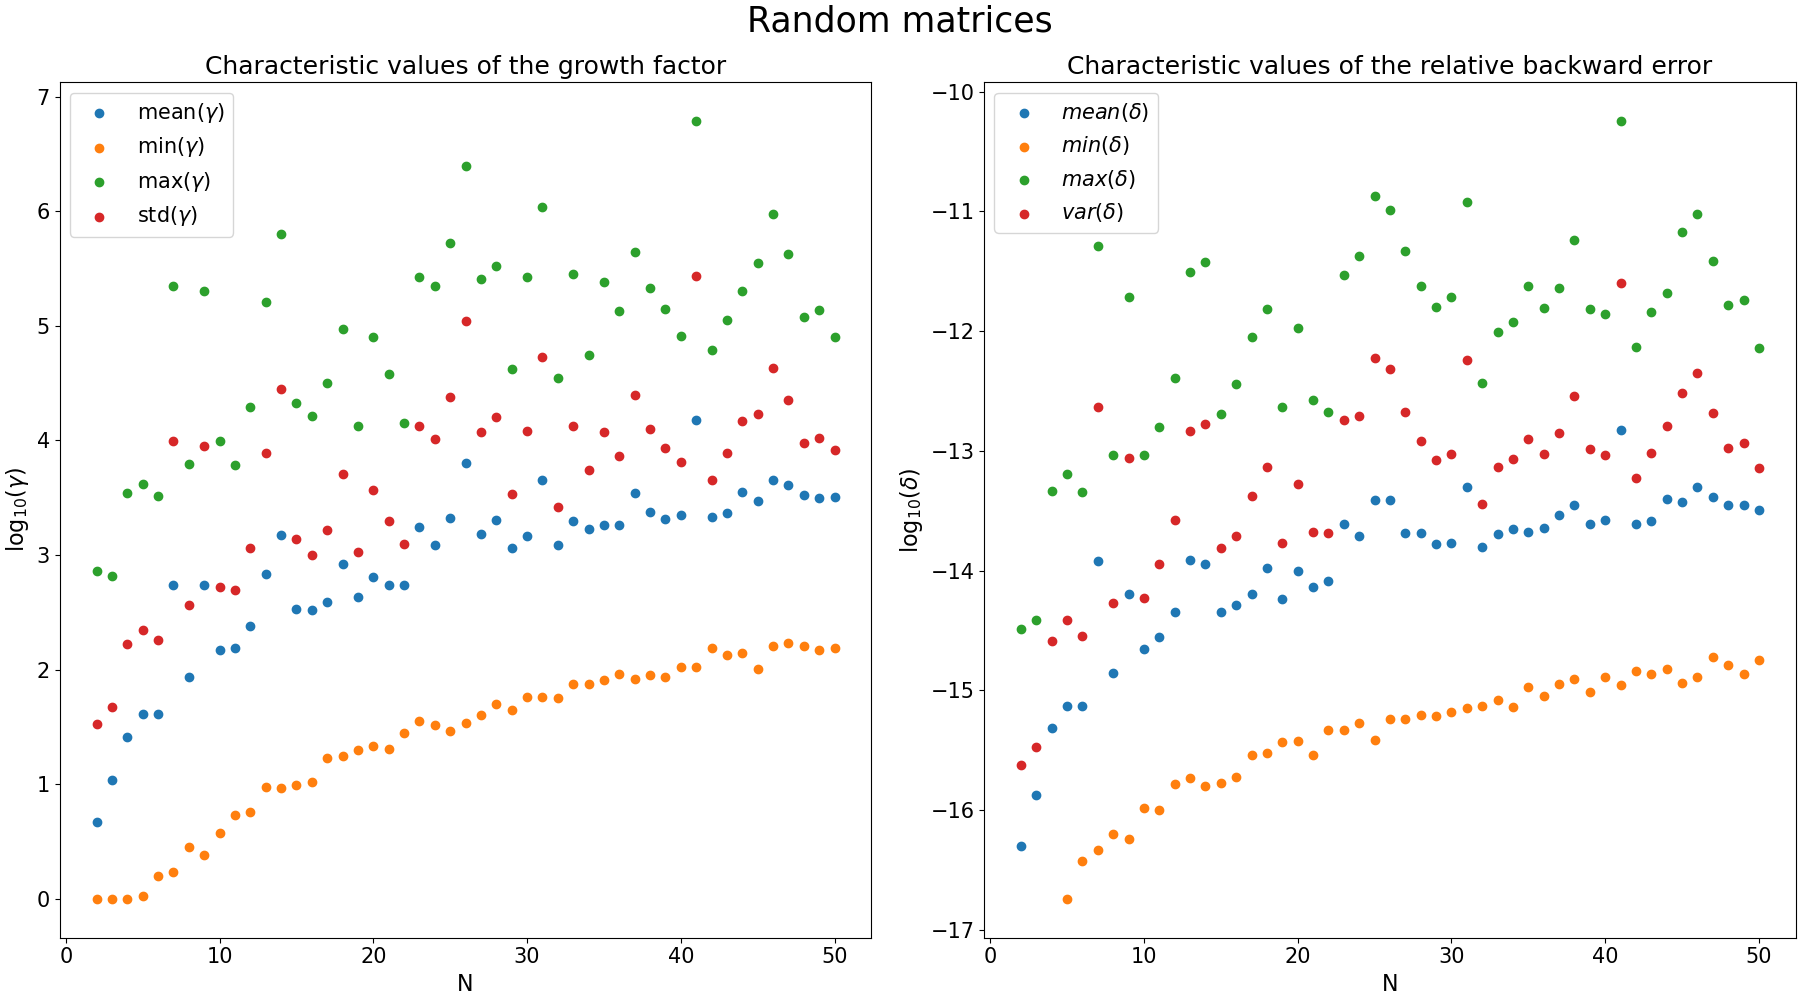
\includegraphics[scale=0.24]{C:/Users/cerra/Documents/GitHub/Numerical_Analysis_Optimization/Project_1_latex/Plot/Scatterplot_charact_values_for_Random_matrices}
	\caption{Scatterplot of the characteristic values of $\gamma$ and $\delta$ as a function of $N$ for real random matrices. Logarithmic scale on the ordinate axis.}
	\label{fig:Scatterplot_Random}
\end{figure}

\begin{figure}[H]
	\centering
	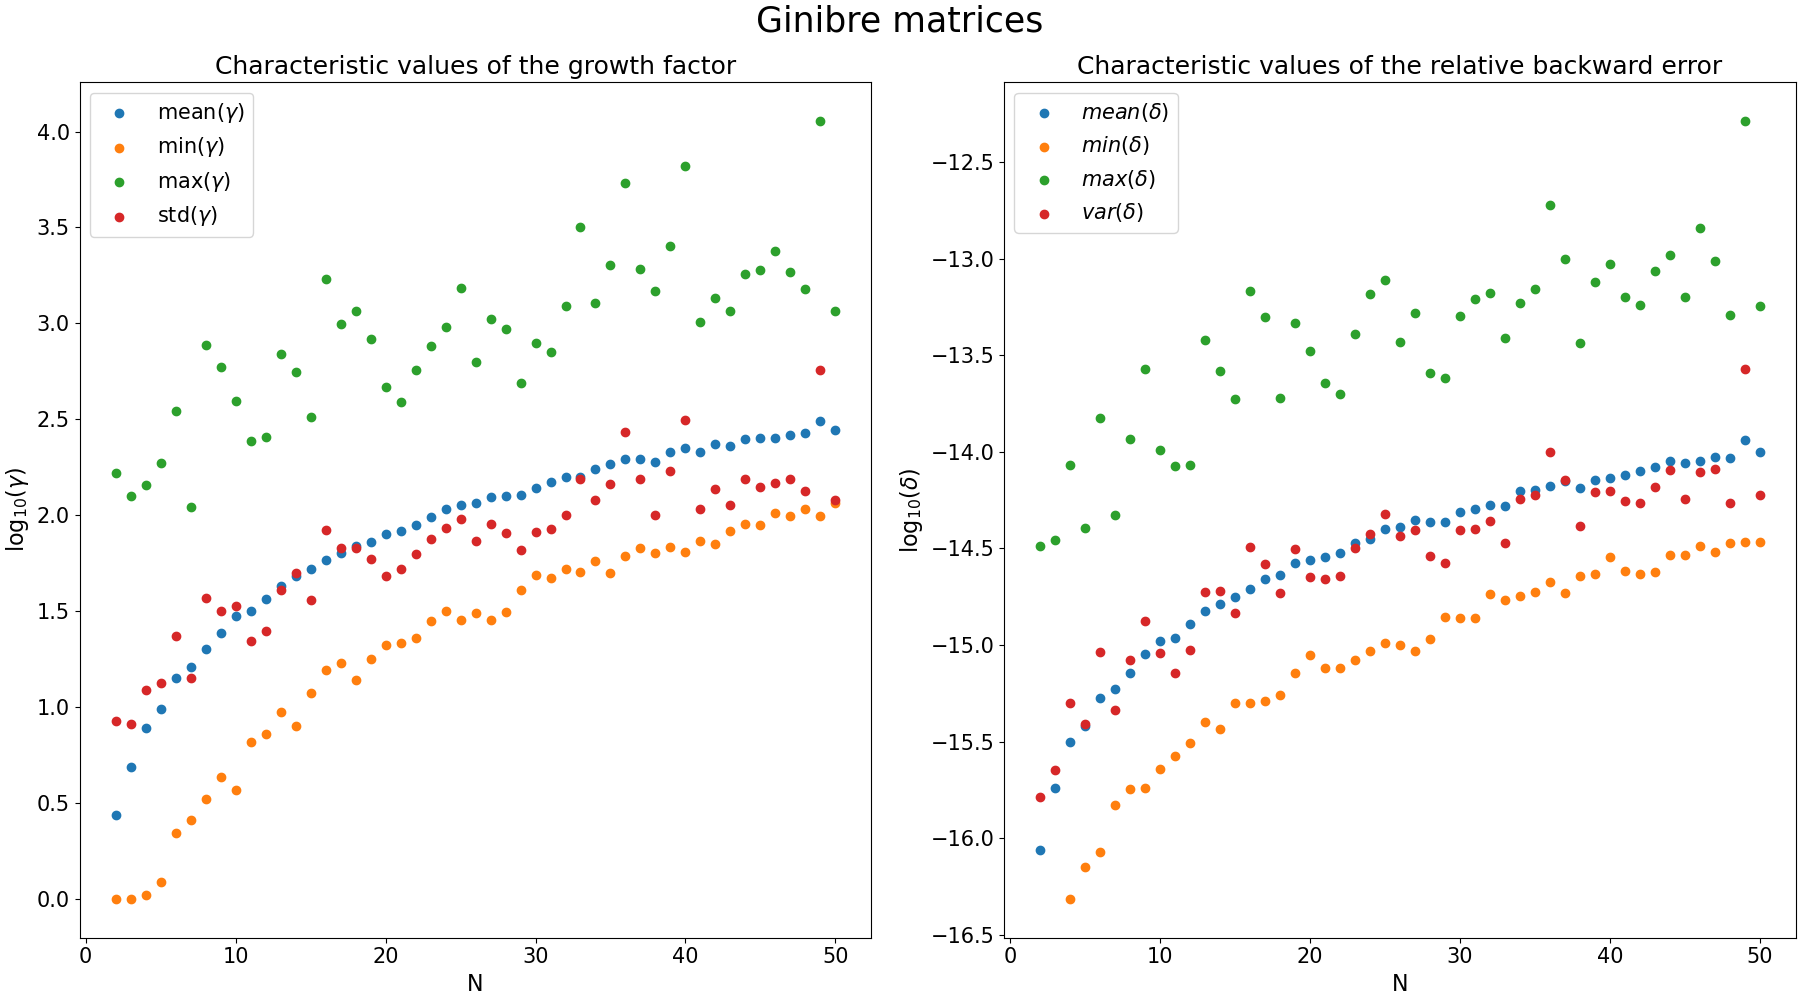
\includegraphics[scale=0.24]{C:/Users/cerra/Documents/GitHub/Numerical_Analysis_Optimization/Project_1_latex/Plot/Scatterplot_charact_values_for_Ginibre_matrices}
	\caption{Scatterplot of the characteristic values of $\gamma$ and $\delta$ as a function of $N$ for Ginibre matrices. Logarithmic scale on the ordinate axis.}
	\label{fig:Scatterplot_Ginibre}
\end{figure}
	
\noindent As can be seen from these plots, the characteristic values of the two considered quantities increase with the dimension of the input matrix for both types of matrices taken into account. This might be due to the fact that, when the dimension of the input matrix increases, the algorithm that performs the LU factorization requires more steps, resulting in a propagation of numerical errors. It is interesting to also consider, for a fixed dimension, the distributions of the growth factor and the relative backward error for both cases. We have chosen to report here the histograms obtained for $N=25$, together with the corresponding boxplots, where the outliers have been removed for clarity of visualization. We have chosen this point as an intermediate representative dimension; similar considerations also hold in the other cases.
\begin{figure}[H]
	\centering
	\subfloat[][]{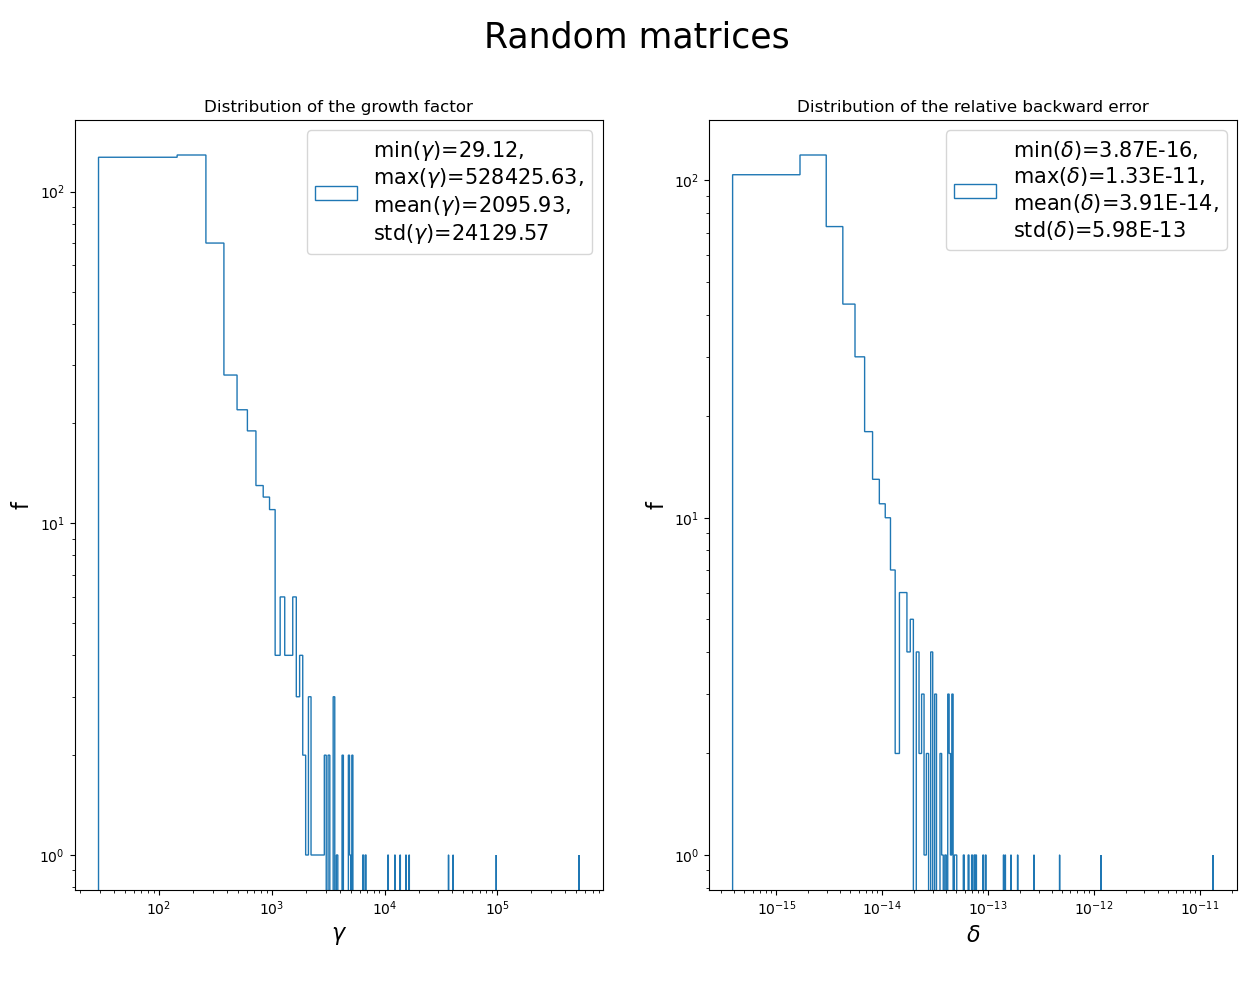
\includegraphics[scale=0.23]{C:/Users/cerra/Documents/GitHub/Numerical_Analysis_Optimization/Project_1_latex/Plot/Distributions_for_Random_matrices_of_dim_25}}\ \subfloat[][]{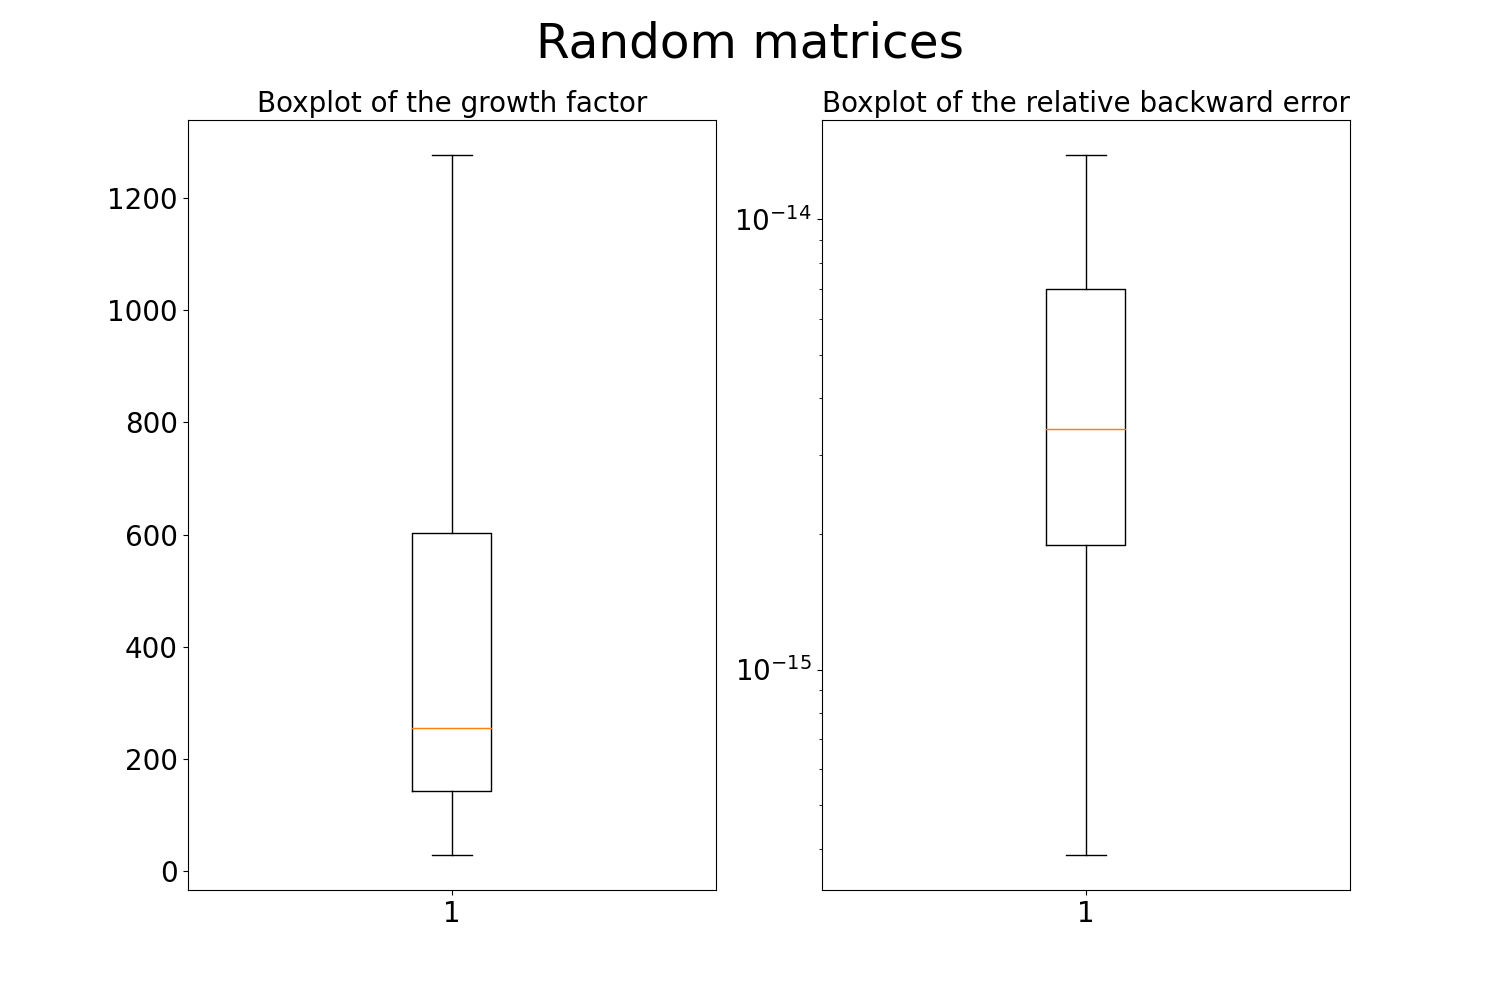
\includegraphics[scale=0.23]{C:/Users/cerra/Documents/GitHub/Numerical_Analysis_Optimization/Project_1_latex/Plot/Boxplot_for_Random_matrices_of_dim_25}}
	\caption{Histograms (panel (a)) and boxplots (panel (b)) of $\gamma$ and $\delta$ considering real random matrices of dimension $25\times 25$. Logarithmic scale is reported on both axis of the histograms as well as on the ordinate axes of the relative backward error boxplot.}
	\label{fig:Distributions and boxplot Random Matrices N=25}
\end{figure}

\begin{figure}[H]
	\centering
	\subfloat[][]{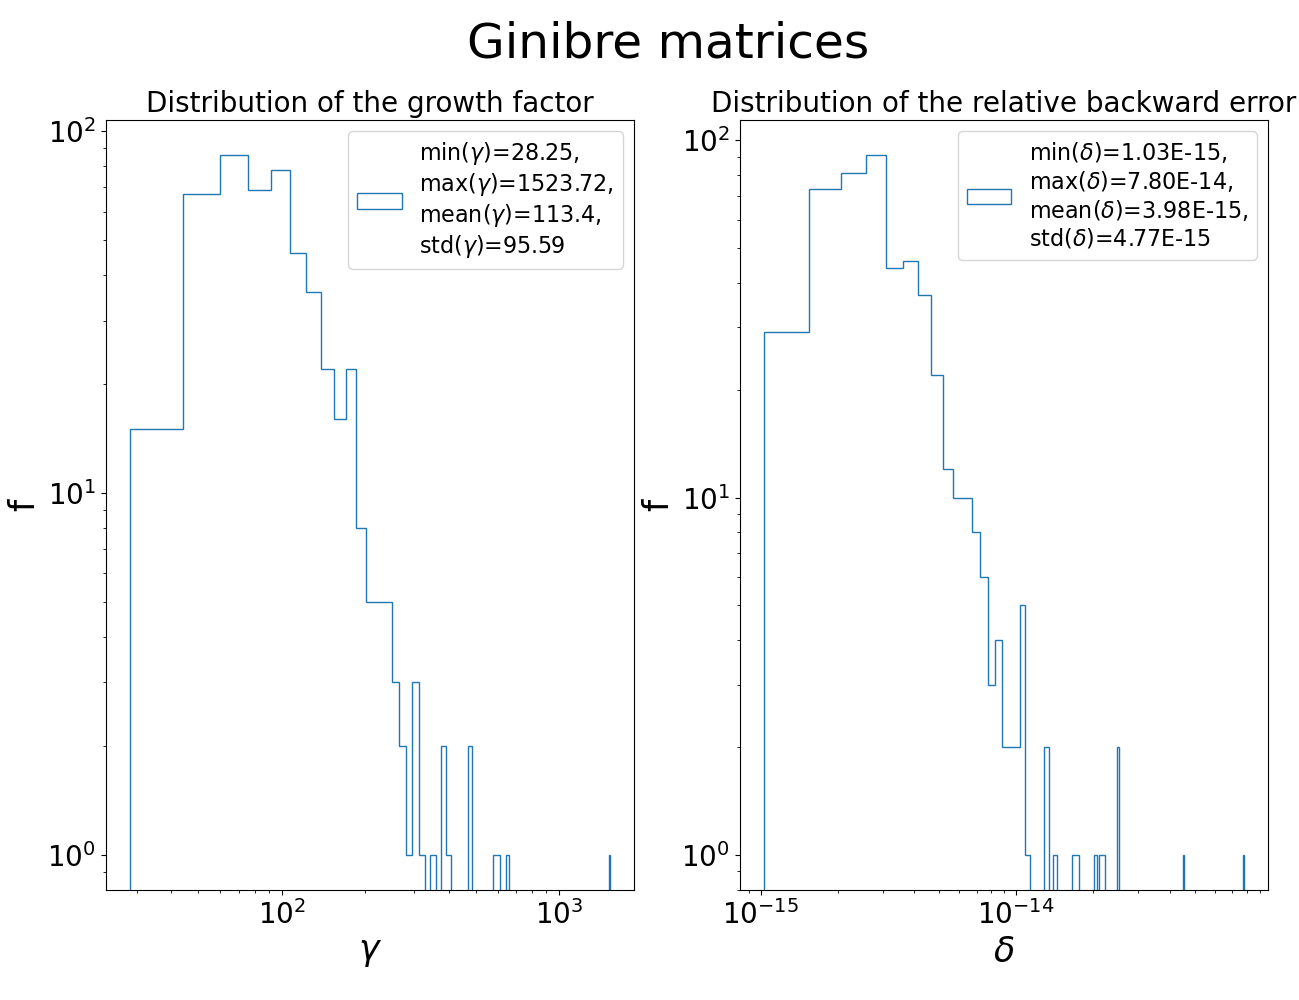
\includegraphics[scale=0.23]{C:/Users/cerra/Documents/GitHub/Numerical_Analysis_Optimization/Project_1_latex/Plot/Distributions_for_Ginibre_matrices_of_dim_25}}\ \subfloat[][]{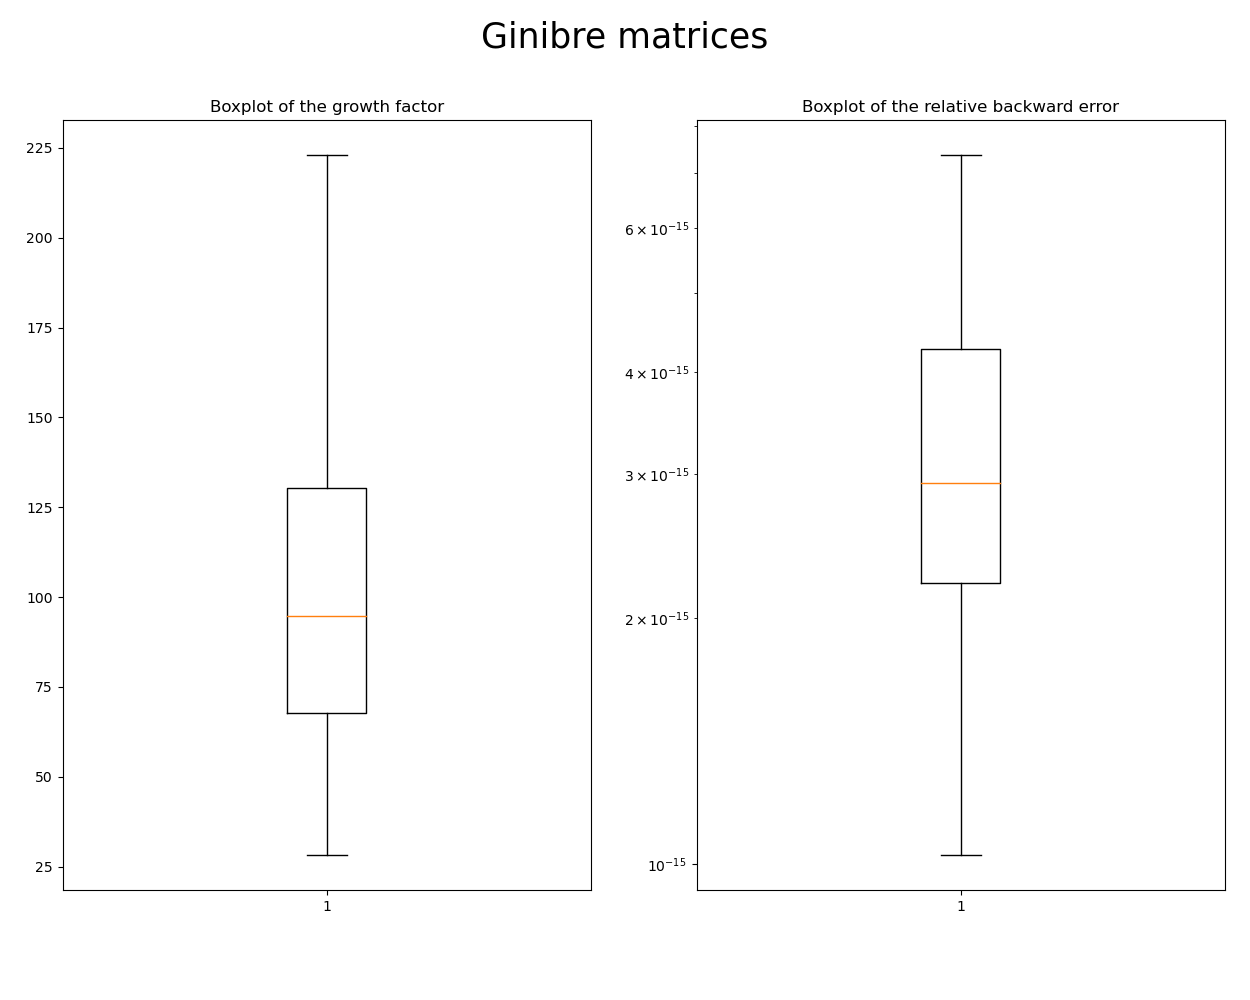
\includegraphics[scale=0.23]{C:/Users/cerra/Documents/GitHub/Numerical_Analysis_Optimization/Project_1_latex/Plot/Boxplot_for_Ginibre_matrices_of_dim_25}}
	\caption{Histograms (panel (a)) and boxplots (panel (b)) of $\gamma$ and $\delta$ considering Ginibre matrices of dimension $25\times 25$. Logarithmic scale is reported on both axis of the histograms as well as on the ordinate axes of the relative backward error boxplot.}
	\label{fig:Distributions and boxplot Ginibre Matrices N=25}
\end{figure}

\noindent It can be observed that both the growth factor and the relative backward error have a wide range of variation, if one also considers outliers, in the case of real random matrices, while these ranges are smaller in the case of Ginibre matrices. This is, in general, an indication of the fact that both quantities strongly depend on the input matrix, even if more careful considerations can be made to distinguish the two types of matrices. In fact, taking into account, for example, the relative backward error and considering also the outliers, one can note that for real random matrices, whose entries are uniformly distributed in $\left[0,1\right)$, this quantity ranges approximatively from $10^{-16}$ to $10^{-11}$. For what concern the Ginibre matrices, the same quantity ranges approximatively from $10^{-15}$ to $10^{-13}$. It is worth noting that the presence of outliers is more marked in the first case.
%However, if one discards the outliers, the range of variation of the relative backward error is approximatively the same in both cases.
This difference in the variation range might be due to the fact that when considering the normal distribution to sample the entries of a random matrix, it is more likely to have matrix elements that are centered in the neighborhood of the mean value, resulting in an ensemble of more homogeneous matrices. This, as a consequence, might reflect in the obtained values of relative backward errors, when computing the LU factorization, which may be similar and with a smaller range of variation. In the other case, when considering the uniform distribution to sample the entries of a random matrix, the resulting ensemble of matrices may be less homogeneous when compared to the previous one, and this might result in a wider range of variation of the quantity under examination. However, even if in both cases the relative backward errors grow with the dimension of the matrix, their values are small enough and, at least for the mean value, not that far from the machine epsilon, that is of order $10^{-16}$. For what concern the growth factor, even if it grows with the dimension of the input matrix, its growth is reasonable as not exponential. Given these considerations, the algorithm can be considered backward stable for these types of matrices.\\

\noindent \textbf{Unitary matrices } We considered in our dataset the ensemble of unitary matrices, namely matrices $U$ such that $U^{*} = U^{-1}$, where $*$ stands for the conjugate transpose. These matrices have been sampled using the \mintinline{Python}{tenpy} Python library and they are also called \textit{CUE matrices}, as they are sampled from the circular ensemble. As in the previous case, we report in the following the scatterplot of the growth factor $\gamma$ and the relative backward error $\delta$ as a function of the dimension $N$ of the matrix.
%We know from theory that the eigenvalues of these matrices are the roots of the unity and, therefore, they all have absolute value equals to one (they are said to be unimodular). 
%For this reason, we expect the LU factorization algorithm to be backward stable
\begin{figure}[H]
	\centering
	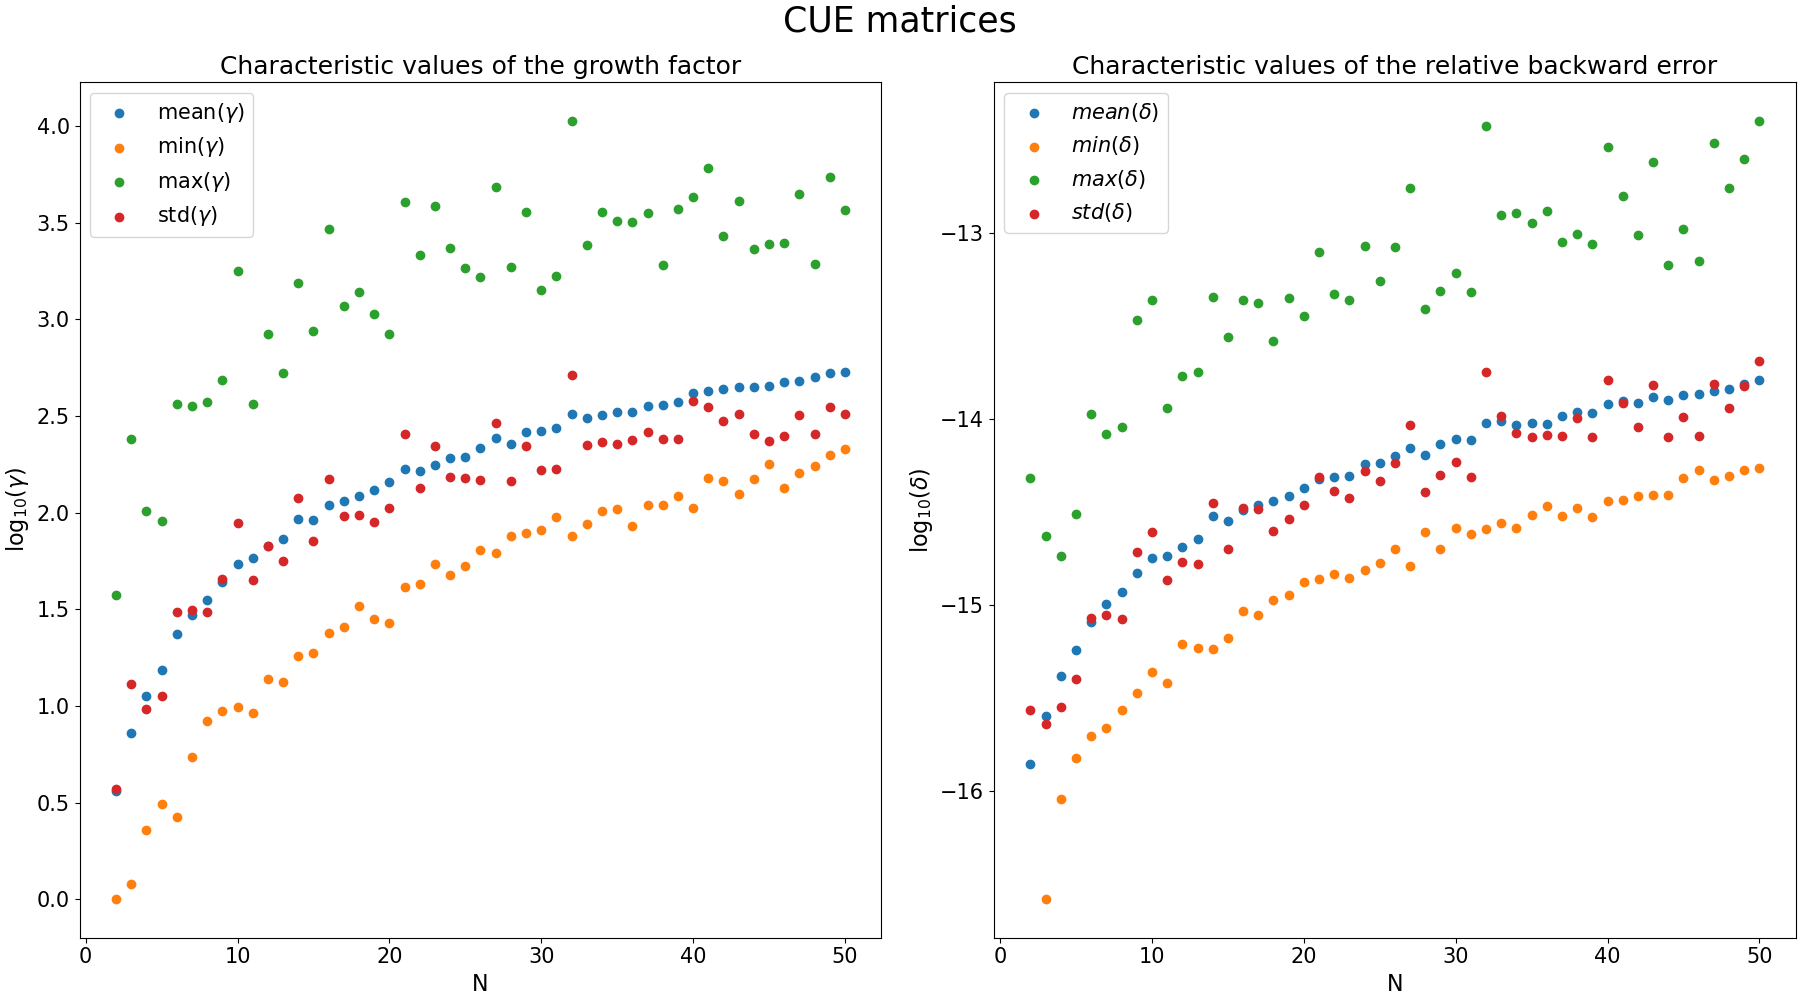
\includegraphics[scale=0.24]{C:/Users/cerra/Documents/GitHub/Numerical_Analysis_Optimization/Project_1_latex/Plot/Scatterplot_charact_values_for_CUE_matrices}
	\caption{Scatterplot of the characteristic values of $\gamma$ and $\delta$ as a function of $N$ for unitary matrices. Logarithmic scale on the ordinate axis.}
	\label{fig:Scatterplot_CUE}
\end{figure}
\noindent  The range of variation of both these quantities is comparable with the one obtained in the case of Ginibre matrices. For this reason, the same considerations regarding the overall stability of the LU factorization algorithm can be made. In fact, as can be seen from the values obtained for $\gamma$ and $\delta$, the LU factorization algorithm can be considered backward stable for unitary matrices.\\
%
%It turns out that this case is quite similar to the case of Ginibre matrices for what concern the range of variation of the characteristic values of both the growth factor and the relative backward error.
%*** This might be understood if one investigates how these matrices are generated in the source code of the \mintinline{Python}{tenpy} library. It can be seen, in fact, that unitary matrices are generated starting from a Ginibre matrix $A$, so a complex matrix whose entries are independent normally distributed, and then performing a QR decomposition, so $A=QR$, where $Q$ is a unitary matrix and $R$ is an upper triangular matrix, and then giving as output a properly rescaled version of the $Q$ matrix. ***
%However, we expect the LU factorization to be backward stable for unitary matrices, and the values of $\gamma$ and $\delta$ that we obtain suggest that this is the case.
%Therefore, it can be concluded that the LU factorization algorithm is backward stable, as expected, for unitary matrices.

\noindent \textbf{Hermitian matrices }  The next class of matrices that we considered is that of Hermitian matrices, namely matrices $H$ such that $H = H^{*}$. In order to sample these matrices we used the \mintinline{Python}{tenpy} Python library. These matrices are also called \textit{GUE matrices} as they are sampled from the Gaussian unitary ensemble.

\begin{figure}[H]
	\centering
	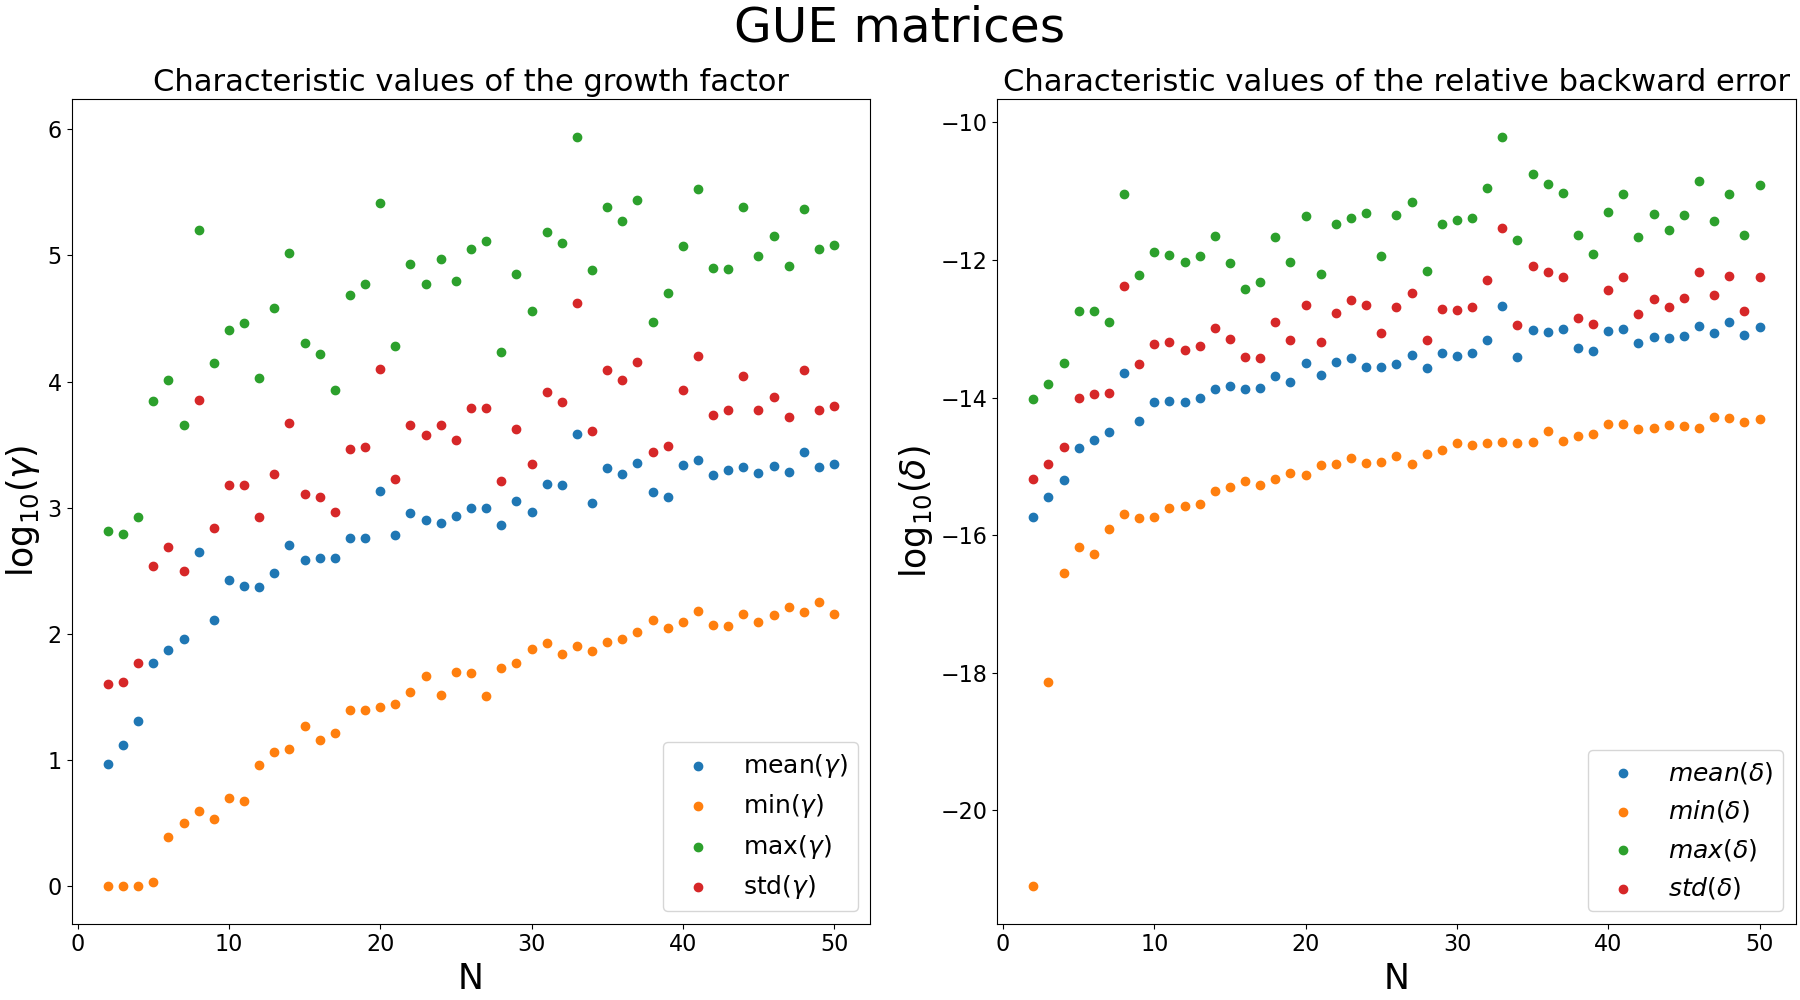
\includegraphics[scale=0.24]{C:/Users/cerra/Documents/GitHub/Numerical_Analysis_Optimization/Project_1_latex/Plot/Scatterplot_charact_values_for_GUE_matrices}
	\caption{Scatterplot of the characteristic values of $\gamma$ and $\delta$ as a function of $N$ for Hermitian matrices. Logarithmic scale on the ordinate axis.}
	\label{fig:Scatterplot_GUE}
\end{figure}

\noindent A characteristic of these scatterplots, as well as of all the others analyzed until now, is that the range of variation of both the growth factor and the relative backward error is quite large, approximatively of three or four orders of magnitude. The choice input matrix has, therefore, an impact in determining these values. However, as in the previous cases, since the trend of the growth factor with the dimension of the input matrix is not exponential and the relative backward error is of the order of the machine precision, these data suggest that the algorithm is backward stable for this class of matrices.\\

\noindent \textbf{Positive definite matrices } The next class of matrices that we considered is that of positive definite matrices. Positive definite matrices $W$ can be obtained by considering matrices of the form $W = A^{*}A$, where $*$ stands for the conjugate transpose, discarding singular matrices. If the matrix $A$ is sampled from the Ginibre ensemble, that is it is a complex matrix whose entries are independent and normally distributed, the matrix $W$ is called \textit{Wishart matrix}. In order to sample these matrices we used the \mintinline{Python}{qutip} Python library, considering, in particular, unit trace matrices. Note that matrices of this kind are also Hermitian. We expect the LU factorization for these matrices to be backward stable.\\

\noindent We report in the following the scatterplot of the growth factor $\gamma$ and the relative backward error $\delta$ as a function of the dimension $N$ of the input matrix.

\begin{figure}[H]
	\centering
	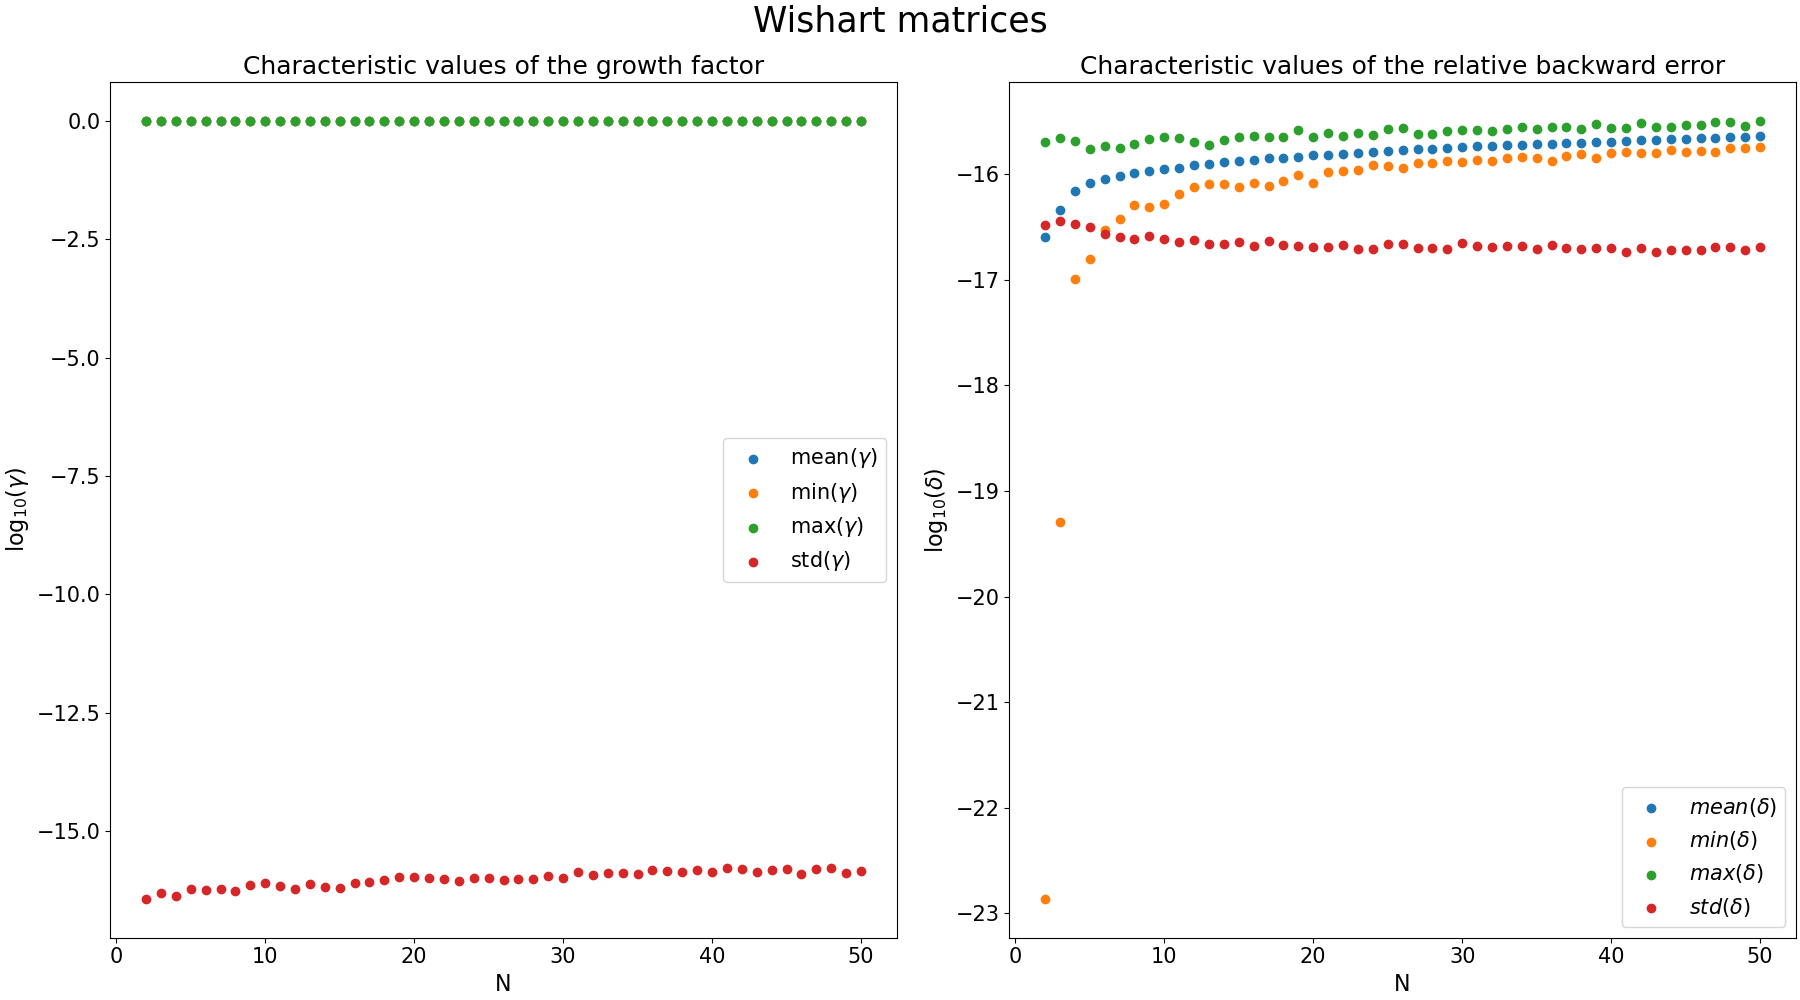
\includegraphics[scale=0.24]{C:/Users/cerra/Documents/GitHub/Numerical_Analysis_Optimization/Project_1_latex/Plot/Scatterplot_charact_values_for_Wishart_matrices}
	\caption{Scatterplot of the characteristic values of $\gamma$ and $\delta$ as a function of $N$ for positive definite matrices. Logarithmic scale on the ordinate axis.}
	\label{fig:Scatterplot_Wishart}
\end{figure}

\noindent It turns out that this case is quite different from the previous ones. In fact, it can be seen that the minimum, maximum, and mean values of the growth factor are all equal to one, while the standard deviation is of the order of the machine epsilon. Moreover, the relative backward error is significantly small and it is of the order of the machine epsilon. It is interesting to note that, in this latter case, the standard deviation is smaller if compared to the other values, suggesting that the distribution of the relative backward error is peaked in correspondence with the mean value. This means that, differently from the other cases, whatever the input matrix, the values obtained for the relative backward error will be approximately the same, or, in other words, they will be included in a very small range. These considerations imply the backward stability of the LU factorization, as expected, for this class of matrices.\\

\noindent \textbf{Diagonally dominant matrices } Another class of matrices that we considered in our dataset is given by the diagonally dominant matrices. These are matrices whose diagonal entries are, in absolute value, greater or equal to the sum of the absolute values of the other elements in the corresponding row, and such that the inequality is strict for at least a row. We have described how we sampled these matrices in the description of the function at the beginning of the chapter. In the following, we report the scatterplot of the growth factor $\gamma$ and the relative backward error $\delta$ as a function of the dimension $N$ of the matrix.

\begin{figure}[H]
	\centering
	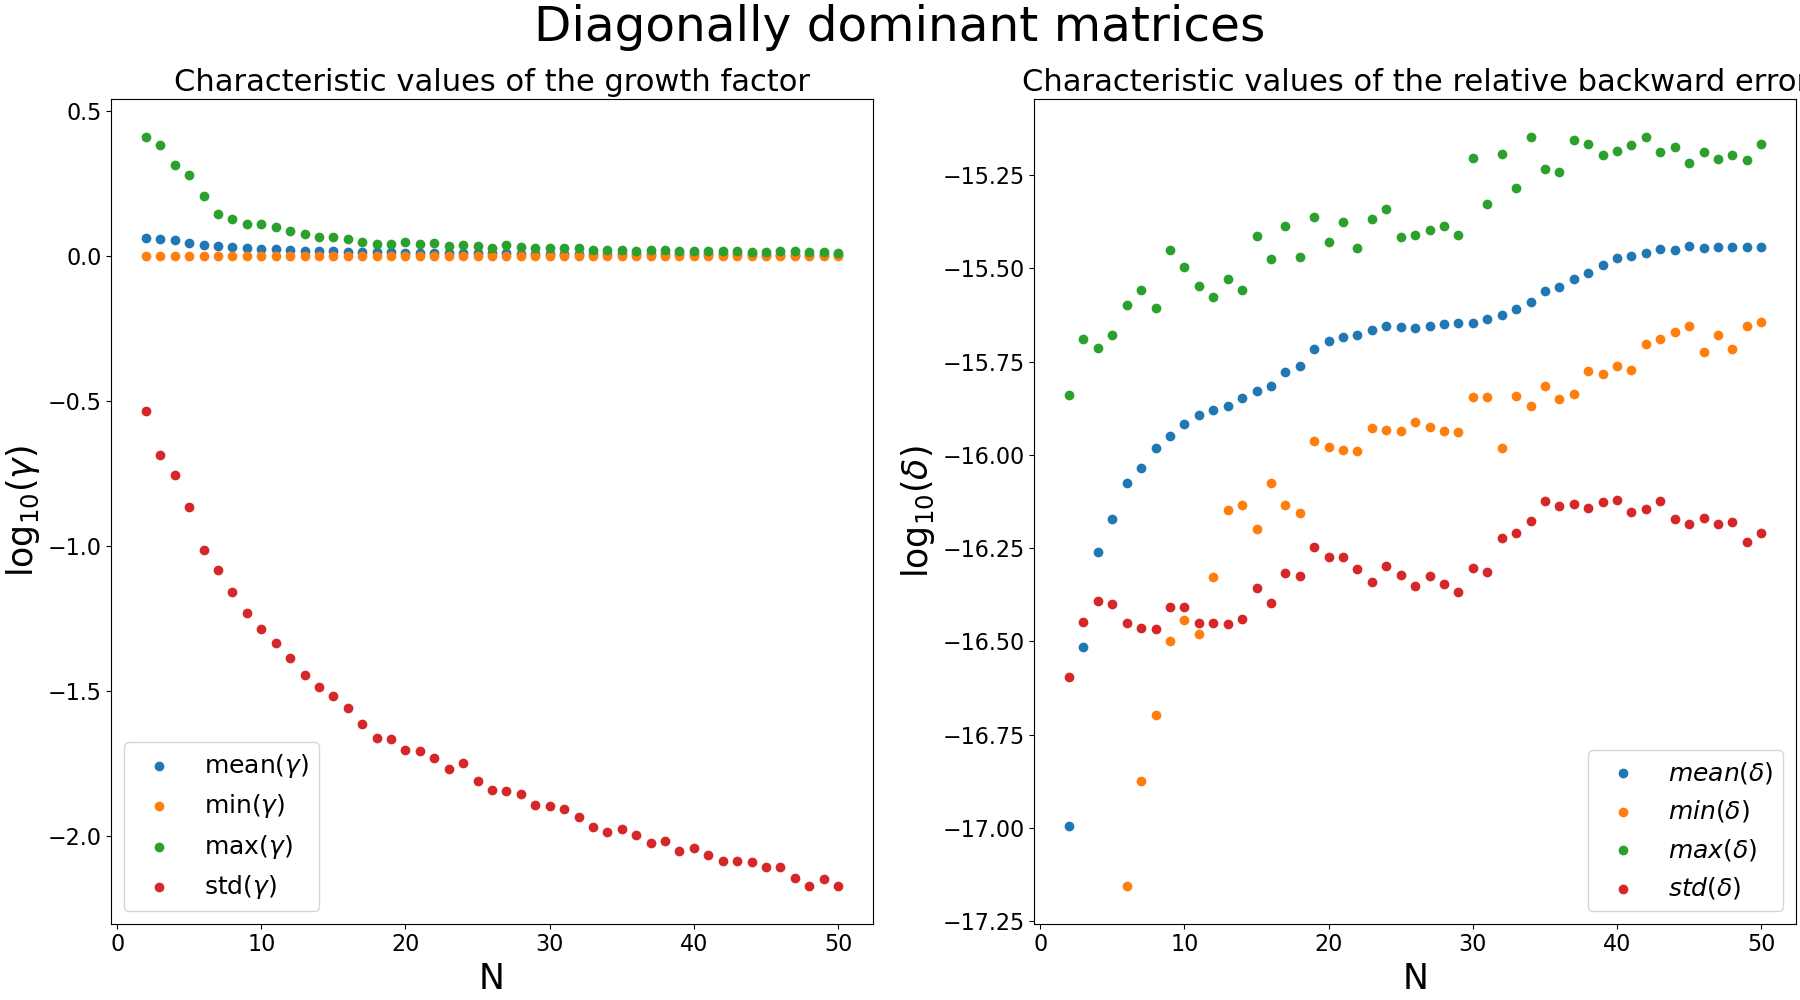
\includegraphics[scale=0.24]{C:/Users/cerra/Documents/GitHub/Numerical_Analysis_Optimization/Project_1_latex/Plot/Scatterplot_charact_values_for_Diagonally dominant_matrices}
	\caption{Scatterplot of the characteristic values of $\gamma$ and $\delta$ as a function of $N$ for diagonally dominant matrices. Logarithmic scale on the ordinate axis.}
	\label{fig:Scatterplot_Diag_dom}
\end{figure}

\noindent In this case, considerations similar to the case of positive definite matrices can be made. In fact, it can be observed that the growth factor is of order $\mathcal{O}(1)$, while the relative backward error is of the order of the machine epsilon, with the standard deviation that suggests, as in the previous case, that the distribution of this quantity, for a fixed dimension of the input matrix, is peaked at the mean value. Therefore, the value obtained for this quantity does not strongly depend on the input matrix. It can be concluded that the LU factorization is backward stable for this class of matrices.\\

\noindent \textbf{Hilbert matrices} In addition to the matrices considered in the dataset, we also analyzed the trend of the growth factor and the relative backward error for the Hilbert matrices $H_{N}$, as a function of their dimension. In this case, it emerges that, when considering a precision given by the unit roundoff $u$, the algorithm that performs the LU factorization breaks for $N\ge26$. In other words, the growth factor is identically equal to one and the relative backward error is of the order of the machine epsilon for $N<26$, while, as $N$ increases, a division by a quantity smaller than the machine epsilon occurs, causing the algorithm to break. This means that the problem of solving a linear system $H_{N}\textbf{x}=\textbf{b}$ is ill-conditioned for $N\ge26$ as its condition number increases. In fact, we know from theory that the condition number of the Hilbert matrix increases exponentially with the dimension of the matrix.

\subsection{Conclusions}
Given the classes of matrices considered in the dataset (which does not include the Hilbert matrices, analyzed separately), we found that the LU factorization is backward stable in all the cases considered, with differences that emerge when comparing the last two types of matrices, namely positive definite matrices and diagonally dominant matrices, to the other ones. In fact, in the last two cases, the values obtained for the relative backward error do not depend on the input matrix, differently from the other cases, where this happens. Moreover, we observed that the LU factorization algorithm never failed, as the DataFrame where we stored all the failures of the algorithm, divided by types of matrix considered and their relative dimension, is identically zero. Different considerations hold for the Hilbert matrices, where the LU factorization algorithm breaks for dimensions of the input matrix greater or equal to $26$ (given the chosen precision), as a consequence of the increasing condition number.

\noindent In the following we report a final plot where we compare the boxplots of all the types of matrices taken into account in the dataset when considering a fixed dimension of the input matrix, that is $N=25$. For greater clarity of visualization, we discard outliers and consider, in this way, the most likely range of possible values.

\begin{figure}[H]
	\centering
	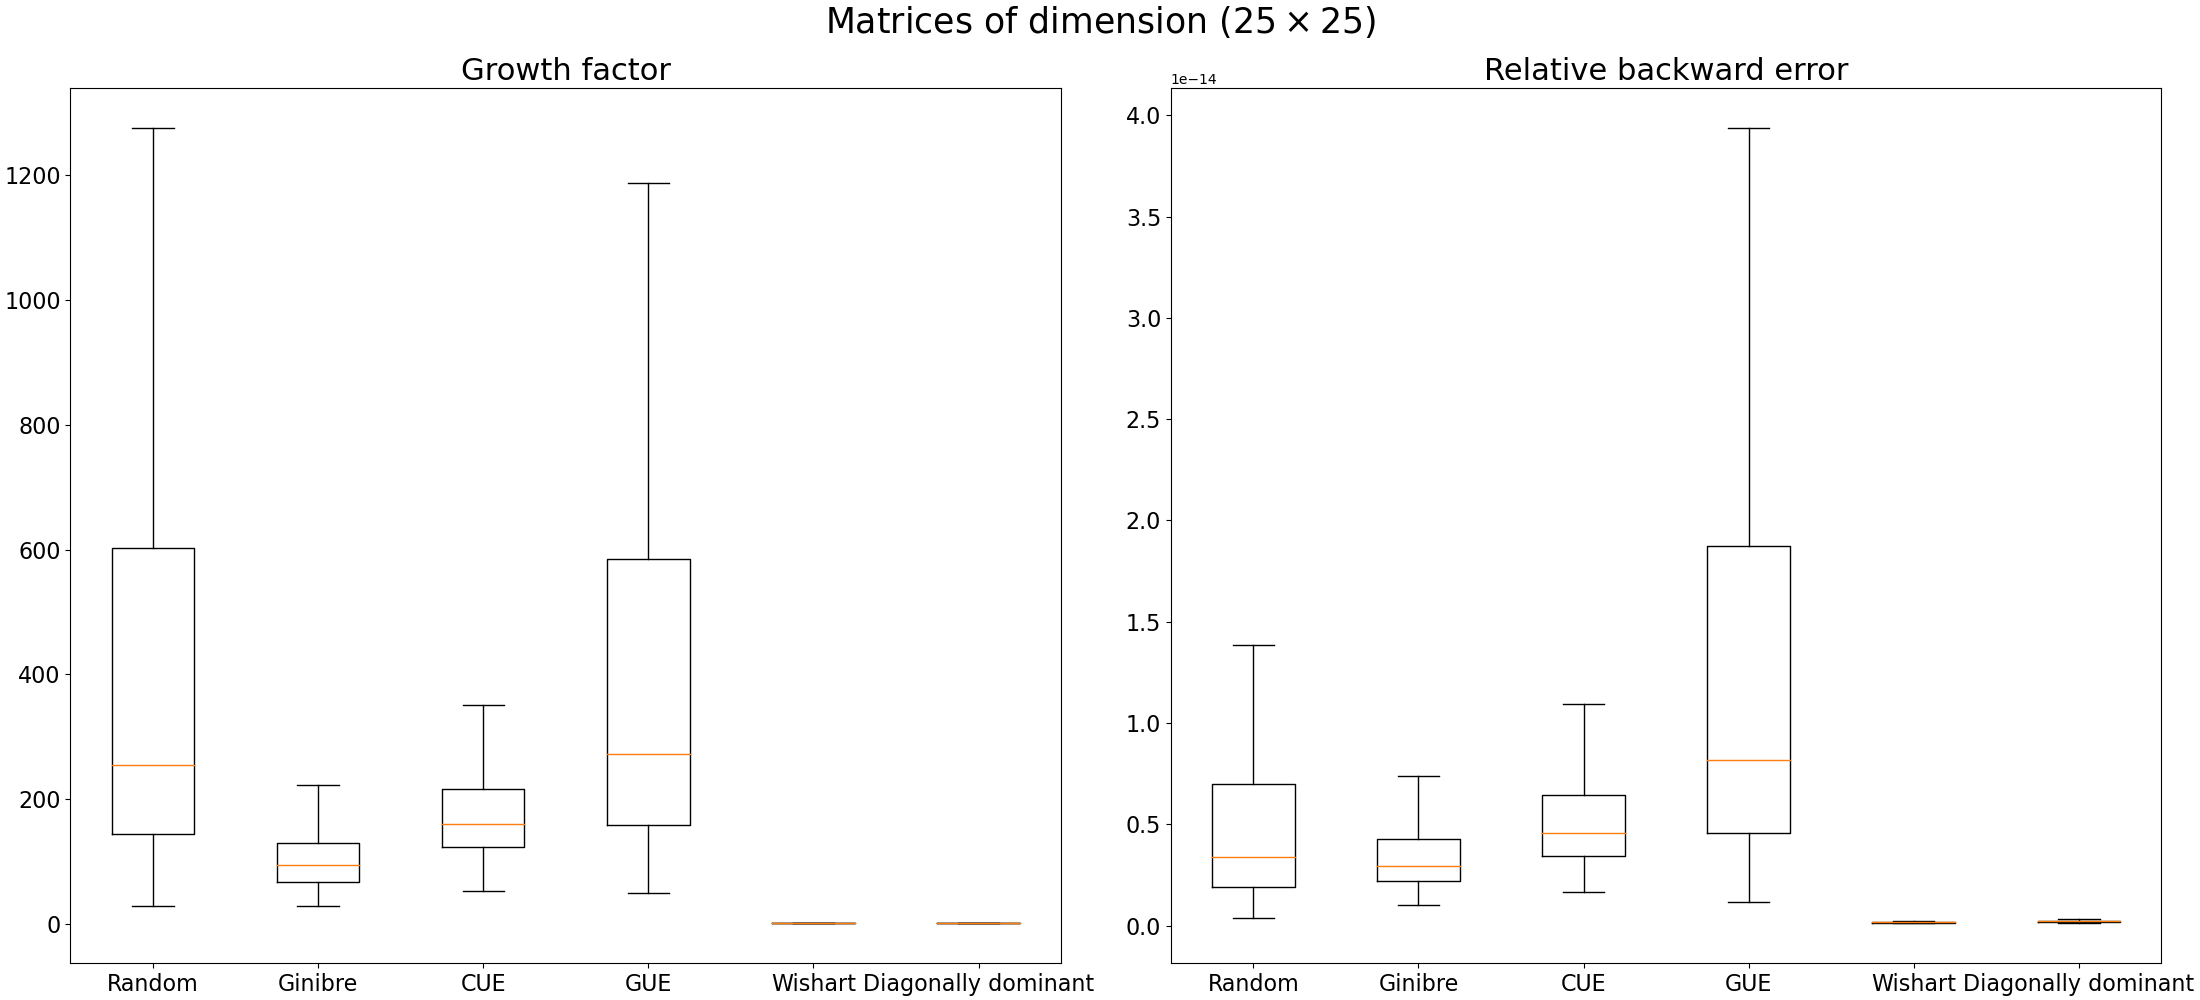
\includegraphics[scale=0.25]{C:/Users/cerra/Documents/GitHub/Numerical_Analysis_Optimization/Project_1_latex/Plot/Boxplot_dim_matr=25}
	\caption{Boxplot of $\gamma$ and $\delta$ for matrices of dimension $25\times25$.}
	\label{fig:Boxplot_final}
\end{figure}

%\newpage
%	Hilbert matrices becomes numerically singular starting from $N=6$, but the LU factorization is still possible (maybe).
%	The LU factorization breaks down for $N=21$ (if one compares the absolute value of the element $A_{kk}$ at the step $k-1$, namely $A_{kk}^{k-1}$, with the machine precision), while it breaks down for $N=15$ if one compares the same two values without considering the absolute value for the first one. What does it mean for us that the LU factorization breaks down? We are comparing the element $A_{kk}^{k-1}$ with the machine precision but maybe this is not the best strategy possible as the relative backward error is still zero, even for larger $N$ values. This is probably due to the fact that such numbers can still be represented in the computer. In fact, the algorithm gives us the correct (maybe) matrices $L$ and $U$ such that $A=LU$f(k).
	
\section{Problem 2}
Consider the $n \times n$ Wilkinson matrix

\begin{equation}\label{key}
	W_n = 
	\begin{bmatrix}
		1 & 0  & 0  & \cdots  & 1  \\
		-1 & 1 & 0 & \cdots & 1 \\
		-1 & -1 & 1 & \cdots & 1 \\
		\vdots & \vdots & \vdots & \ddots & \vdots \\
		-1 & -1 & \cdots & -1 & 1 
	\end{bmatrix}
\end{equation}

\noindent \textbf{(1)} We are interested to compute (by hand) the LU factorization of $W_{5}$, therefore to compute two $n \times n$ matrices, $L_5$ and $U_5$, that are, respectively, a unit lower triangular matrix and an upper triangular matrix that satisfy the identity $W_5 = L_5 U_5$. We start writing the expression of $W_5$:
\begin{equation}\label{key}
	W_5 = 
	\begin{bmatrix}
		1 & 0  & 0  & 0  & 1  \\
		-1 & 1 & 0 & 0 & 1 \\
		-1 & -1 & 1 & 0 & 1 \\
		-1 & -1 & -1 & 1 & 1 \\
		-1 & -1 & -1 & -1 & 1 
	\end{bmatrix},
\end{equation}
now we compute $\textbf{m}_1$:
\begin{equation}\label{key}
	\textbf{m}_1 = 
	\begin{bmatrix}
		0\\
		{w_{21}}/{w_{11}}\\
		{w_{31}}/{w_{11}}\\
		{w_{41}}/{w_{11}}\\
		{w_{51}}/{w_{11}}
	\end{bmatrix}=
	\begin{bmatrix}
		0\\
		-1\\
		-1\\
		-1\\
		-1
	\end{bmatrix}.
\end{equation}
Defining $\textbf{e}_i$ as the vectors with $1$ in the $i-th$ element and $0$ otherwise, we can compute:
\begin{equation}\label{key}
	M_1=\mathcal{I}_5 - \textbf{m}_1 \textbf{e}_1^T =
	\begin{bmatrix}
		1 & 0  & 0  & 0  & 0  \\
		1 & 1 & 0 & 0 & 0\\
		1 & 0 & 1 & 0 & 0 \\
		1 & 0 & 0 & 1 & 0 \\
		1 & 0 & 0 & 0 & 1 
	\end{bmatrix}.
\end{equation}
Using the expression of $M_1$, we can compute $W_5^{(1)}$:
\begin{equation}\label{key}
	W_5^{(1)} = M_1 W_5 = 
	\begin{bmatrix}
		1 & 0  & 0  & 0  & 1  \\
		0 & 1 & 0 & 0 & 2 \\
		0 & -1 & 1 & 0 & 2 \\
		0 & -1 & -1 & 1 & 2 \\
		0 & -1 & -1 & -1 & 2 
	\end{bmatrix}.
\end{equation}
The second iteration proceeds in a similar way:
\begin{equation}\label{key}
	\textbf{m}_2 = 
	\begin{bmatrix}
		0\\
		0\\
		{w^{(1)}_{32}}/{w^{(1)}_{22}}\\
		{w^{(1)}_{42}}/{w^{(1)}_{22}}\\
		{w^{(1)}_{52}}/{w^{(1)}_{22}}
	\end{bmatrix}=
	\begin{bmatrix}
		0\\
		0\\
		-1\\
		-1\\
		-1
	\end{bmatrix},
\end{equation}

\begin{equation}\label{key}
	M_2=\mathcal{I}_5 - \textbf{m}_2\textbf{e}_2^T =
	\begin{bmatrix}
		1 & 0  & 0  & 0  & 0  \\
		0 & 1 & 0 & 0 & 0\\
		0 & 1 & 1 & 0 & 0 \\
		0 & 1 & 0 & 1 & 0 \\
		0 & 1 & 0 & 0 & 1 
	\end{bmatrix}.
\end{equation}

\noindent Using the expression of $M_2$, we can compute $W_5^{(2)}$:
\begin{equation}\label{key}
	W_5^{(2)} = M_2 W_5^{(1)} = M_2 M_1 W_5 =
	\begin{bmatrix}
		1 & 0  & 0  & 0  & 1  \\
		0 & 1 & 0 & 0 & 2 \\
		0 & 0 & 1 & 0 & 4 \\
		0 & 0 & -1 & 1 & 4 \\
		0 & 0 & -1 & -1 & 4 
	\end{bmatrix}.
\end{equation}

\noindent Now we start the third iteration:
\begin{equation}\label{key}
	\textbf{m}_3 = 
	\begin{bmatrix}
		0\\
		0\\
		0\\
		{w^{(2)}_{43}}/{w^{(2)}_{33}}\\
		{w^{(2)}_{53}}/{w^{(2)}_{33}}
	\end{bmatrix}=
	\begin{bmatrix}
		0\\
		0\\
		0\\
		-1\\
		-1
	\end{bmatrix},
\end{equation}

\begin{equation}\label{key}
	M_3=\mathcal{I}_5 - \textbf{m}_3\textbf{e}_3^T =
	\begin{bmatrix}
		1 & 0  & 0  & 0  & 0  \\
		0 & 1 & 0 & 0 & 0\\
		0 & 0 & 1 & 0 & 0 \\
		0 & 0 & 1 & 1 & 0 \\
		0 & 0 & 1 & 0 & 1 
	\end{bmatrix}.
\end{equation}

\noindent Using the expression of $M_3$, we can compute $W_5^{(3)}$:
\begin{equation}\label{key}
	W_5^{(3)} = M_3 W_5^{(2)} = M_3 M_2 M_1 W_5 =
	\begin{bmatrix}
		1 & 0  & 0  & 0  & 1  \\
		0 & 1 & 0 & 0 & 2 \\
		0 & 0 & 1 & 0 & 4 \\
		0 & 0 & 0 & 1 & 8 \\
		0 & 0 & 0 & -1 & 8 
	\end{bmatrix}.
\end{equation}

\noindent Similarly, we can perform the last iteration:
\begin{equation}\label{key}
	\textbf{m}_4 = 
	\begin{bmatrix}
		0\\
		0\\
		0\\
		0\\
		{w^{(2)}_{54}}/{w^{(2)}_{44}}
	\end{bmatrix}=
	\begin{bmatrix}
		0\\
		0\\
		0\\
		0\\
		-1
	\end{bmatrix},
\end{equation}

\begin{equation}\label{key}
	M_4=\mathcal{I}_5 - \textbf{m}_4\textbf{e}_4^T =
	\begin{bmatrix}
		1 & 0  & 0  & 0  & 0  \\
		0 & 1 & 0 & 0 & 0\\
		0 & 0 & 1 & 0 & 0 \\
		0 & 0 & 0 & 1 & 0 \\
		0 & 0 & 0 & 1 & 1 
	\end{bmatrix}.
\end{equation}

\noindent Using the expression of $M_4$, we can compute $W_5^{(4)}$:
\begin{equation}\label{key}
	W_5^{(4)} = M_4 W_5^{(3)} = M_4 M_3 M_2 M_1 W_5 =
	\begin{bmatrix}
		1 & 0  & 0  & 0  & 1 \\
		0 & 1 & 0 & 0 & 2 \\
		0 & 0 & 1 & 0 & 4 \\
		0 & 0 & 0 & 1 & 8 \\
		0 & 0 & 0 & 0 & 16 
	\end{bmatrix} = U_5.
\end{equation}
Since this last matrix is upper triangular, we call it $U_{5}$ and define $L^{-1}_{5} \coloneqq M_4 M_3 M_2 M_1$, such that $L^{-1}_{5}W_{5}= U_{5}$. We can get $L_5$ from $L_5 = M_1^{-1} M_2^{-1} M_3^{-1} M_4^{-1}$ and knowing that $M_i^{-1} = \mathcal{I}_5 + \textbf{m}_i \textbf{e}_i^T$:
\begin{equation}\label{key}
	L_5 = M_1^{-1} M_2^{-1} M_3^{-1} M_4^{-1} = 
	\begin{bmatrix}
		1 & 0  & 0  & 0  & 0  \\
		-1 & 1 & 0 & 0 & 0 \\
		-1 & -1 & 1 & 0 & 0 \\
		-1 & -1 & -1 & 1 & 0 \\
		-1 & -1 & -1 & -1 & 1 
	\end{bmatrix}.
\end{equation}

\noindent \textbf{(2)} It is possible to guess the LU factorization of $W_n = L_n U_n$:
\begin{equation}\label{key}
	L_n =
	\begin{bmatrix}
		1 & 0  & \cdots  & \cdots  & 0 \\
		-1 & 1 & \ddots & \  & \vdots \\
		\vdots & \ddots & 1 & \ddots & \vdots \\
		\vdots & \  & \ddots & \ddots & 0 \\
		-1 & \cdots & \cdots & -1 & 1 
	\end{bmatrix},\ \ \ 
	U_n = 
	\begin{bmatrix}
		1 & 0  & \cdots  & 0  & 2^0 \\
		0& 1 & \ddots & \vdots & 2^1 \\
		\vdots & \ddots & \ddots & 0 & 2^2 \\
		\vdots & \  & \ddots & 1 & \vdots \\
		0 & \cdots & \cdots & 0 & 2^{n-1}
	\end{bmatrix}
\end{equation}


\noindent \textbf{(3)} In the following, we report the function that generates the $n \times n $ Wilkinson matrix.
\begin{minted}[linenos, breaklines]{python}
def wilkin(n):
 r''' This function computes the Wilkinson matrix of dimension :math:`(n \times n)`.
 
 Parameters
 -----------
 n : int
     Dimension of the Wilkinson matrix
 
 Returns
 --------
 W : ndarray
     Wilkinson matrix
 '''
 W = np.tril(-np.ones((n,n)),k=-1) + np.eye(n)
 W[:,n-1] = 1
 return W
\end{minted}
\noindent \textbf{(4-5-6)} In the following, we report the code that performs the numerical experiment for each $n=2,\dots,60$.

\begin{minted}[linenos, breaklines]{python}
def check_when_lufact_W_fails(n_max = 60, threshold = np.finfo(float).eps):
 r''' This function checks the failures of GEPP for a Wilkinson matrix W_n with dimension less or equal to n_max. We define a failure as a case in which the error between the solution found by the algorithm and the expected solution is higher than a chosen threshold. The default threshold is set equal to the machine epsilon. When an error is found, a warning message is printed. The function returns the list of the dimensions less than or equal to n_max for which the GEPP algorithm fails.

 Parameters
 -----------
 n_max : int
         Maximum dimension of the Wilkinson matrix

 Returns
 --------
 fails : list
         List of dimensions for which the algorithm fails
'''

 fails = []

 # Cycle on the dimension of the input
 for n in range(2,n_max+1):
    W = wilkin(n)
    logging.debug(f'W = {W}')

    # Define the vector b
    vect = np.ones(n)
    b = W @ vect

    # Solve the system with GEPP
    x = np.linalg.solve(W,b)

    # Compute the error in 1-norm between the computed solution and the exact solution, and print a warning message when the error exceeds the chosen precision
    error = sum(np.abs(x - vect))
    if error <= threshold:
      logging.info(f'n = {n}, ||x - e||_1 = {error}')
    elif error > threshold:
      logging.warning(f'n = {n}, ||x - e||_1 = {error}')
      fails.append(n)
      # Cycle on the elements of the computed solution and print a warning message with the wrong elements of the solution.
      for i in range(n):
         if abs(x[i] - 1) > threshold:
            logging.warning(f'x[{i}] = {x[i]}')
return fails

\end{minted}

\noindent We have seen that the largest value of $n$ for which $W_n \textbf{x} = \textbf{b}$ can be solved accurately is $54$, that means that for $n=55$ the program returns an inaccurate value for the solution $\textbf{x}$. In particular, instead of computing the value $\textbf{x} = \textbf{e} = [1,\dots,1]^T$, it computes $\tilde{\textbf{x}} = [1,\dots,1,0,1]^T$. In other words, we have:
\begin{equation}\label{key}
	\tilde{\textbf{x}}_{54} = 0 \neq \textbf{e}_{54} = 1.
\end{equation}
In order to understand why this happens, we have verified that the matrices $L_{55}$ and $U_{55}$ are computed accurately. This is done in the function \mintinline{Python}{compute_error_lufact_W(n)}, which can be found in the library \href{https://github.com/nunziacerrato/Numerical_Analysis_Optimization/blob/main/Project_1/Project_1.py}{Project\_1}. In this way, we know that the problem must be in the calculation of the forward and backward substitution. Note that having performed the LU factorization of the matrix $W_{55}$ allows us to solve the system $W_{55} \textbf{x} = \textbf{b}_{55}$ by solving (in order) the following two linear systems with forward and backward substitutions:
\begin{equation}\label{key}
	\left\lbrace \begin{split}
		& L \textbf{y} = \textbf{b} \\
		& U \textbf{x} = \textbf{y}
	\end{split} \right. \ ,
\end{equation}
where we named $L_{55} = L$, $U_{55} = U$, and $\textbf{b}_{55} = \textbf{b}$ for clarity.
It can be verified that the analytical solution to the first system is $\textbf{y} = [2^0 + 1, 2^1 + 1, \dots,2^{n-2}+1, 2^{n-1}]$. At this point, an important observation arises: if we consider $\textbf{y}_{54}$ = $2^{53} + 1 $, we may notice that, when the sum $2^{53} + 1$ is performed in double precision, the result is $2^{53}$. This happens because, in double precision, $\text{fl}(2^{53}+1)=2^{53}$ or, in other words, 1 is smaller than the numerical distance between $2^{53}$ and the next representable number, when working in double precision. This can be justified by estimating the absolute error associated with the representation of $2^{53}+1$:
%This is justified by the fact that:
%$1$ is less than the machine precision associated to the number $2^{53}$, written in double precision:
%\begin{equation}\label{key}
%	1< 2^{53} \cdot \varepsilon \simeq 2^{53} \cdot 2.22 \cdot 10^{-16} \simeq 0.9 \cdot 10^{16} \cdot 2.22 \cdot 10^{-16} \simeq 2.
%\end{equation}
\begin{equation}
	|x - \text{fl}(x)| < u |x| = 2^{-53}(2^{53}+1) = 1 + 2^{-53}.
\end{equation}
After having computed $\textbf{y}$, we can compute the solution of the second system starting from the bottom:
\begin{equation}\label{key}
	x_{55} = y_{55}/U_{55,55} = \frac{2^{54}}{2^{54}} = 1.
\end{equation}
Now we update the vector $\textbf{y}$ as follows:
\begin{equation}\label{key}
	\textbf{y}^{(1)} = \textbf{y} - x_{55} \textbf{u}_{55},
\end{equation}
where $\textbf{u}_{55}$ is the $55-th$ and last column of $U$. The $54-th$ component of $\textbf{y}^{(1)}$ will be:
\begin{equation}\label{key}
	[\textbf{y}^{(1)}]_{54} = [\textbf{y}]_{54} - x_{55} U_{54,55} = 2^{53} + 1 - 2^{53},
\end{equation}
but, since in double precision we have $ 2^{53} + 1 = 2^{53}$, the returned value of  $[\textbf{y}^{(1)}]_{54}$ will be $0$ and not $1$. If we execute the same algorithm for bigger values of $n$, the number of elements of the solution vector that will be miscalculated will grow, starting from the penultimate element of the vector $\textbf{x}$. It is worth noting that the last element of the solution is not affected by this kind of error because it is computed via the operation:
\begin{equation}\label{key}
	x_{n} = y_{n}/U_{n,n} = \frac{2^{n-1}}{2^{n-1}},
\end{equation}
that does not lead to catastrophic cancellations. These considerations imply that the GEPP algorithm is not backward stable when the input is a Wilkinson matrix. However, it is important to say that this is a very artificial example where the growth factor $\gamma$ assumes the maximum possible value, i.e. $\gamma = 2^{n-1}$. However, in most cases, the GEPP algorithm is backward stable.\\

\noindent For the sake of completeness, we have developed a function, named \mintinline{Python}{step_by_step_GEPP_W(n)} that calculates step by step the forward and backward substitution using the GEPP algorithm for Wilkinson matrices, commented in such a way as to make each step explicit, with warnings that signal errors due to catastrophic cancellations.

\section{Problem 3}
Suppose that $A \in \R^{n \times n}$ is a nonsingular matrix and the LU factorization of $A$ exists and has been computed. Consider two given vectors $\textbf{u},\textbf{v}\in \R^n$, we can define the matrix $\tilde{A} = A + \textbf{u}\textbf{v}^T$.\\

\noindent \textbf{(1a)} Prove that $\tilde{A}$ is nonsingular if and only if $\textbf{v}^TA^{-1}\textbf{u} \neq - 1$.\\

\noindent Proof: We start proving that $\det(\tilde{A})\neq 0 $ implies that $\textbf{v}^TA^{-1}\textbf{u} \neq - 1$. We can choose an orthonormal basis $\mathcal{B} =\{\mathbf{e}_i\}_{i=1,\dots,n}$ of $\R^n$ such that $\mathbf{u} = \alpha_1 \mathbf{e}_1$ and $\mathbf{v} = \beta_1 \mathbf{e}_1 + \beta_2 \mathbf{e}_2$ with $\alpha_1, \beta_1, \beta_2 \in \R$. We can represent the matrix $A$ with respect to the basis $\mathcal{B}$, denoting with $a_{ij} = \textbf{e}^T_i A \textbf{e}_j $  the element of the $i-th$ row and $j-th$ column of the matrix $A$ written in the basis $\mathcal{B}$. We can represent the matrix $ \textbf{u}\textbf{v}^T$ with respect to the basis $\mathcal{B}$, obtaining $\textbf{u}\textbf{v}^T = \alpha_1 \beta_1 \textbf{e}_1 \textbf{e}_1^T +  \alpha_1 \beta_2 \textbf{e}_1 \textbf{e}_2^T$. It is known that we can compute the determinant of a $n\times n$ matrix $M$ using the formula
\begin{equation}\label{key}
	\det(M) = \sum_{j=1}^{n} m_{ij} C_{ij}(M),
\end{equation}
where $C_{ij}$ is the cofactor of the element $(i,j)$ of the matrix $M$. Therefore, the determinant of $\tilde{A}$ is:
\begin{equation}\label{key}
	\det(\tilde{A}) = \det(A) + \alpha_1 \beta_1 C_{11}(A) + \alpha_1 \beta_2 C_{12}(A).
\end{equation}
Since we know that $ \det(\tilde{A}) \neq 0$, we can write:
\begin{equation}\label{key}
	\det(A) + \alpha_1 \beta_1 C_{11}(A) + \alpha_1 \beta_2 C_{12}(A) \neq 0,
\end{equation}
and, therefore:
\begin{equation}\label{key}
	\alpha_1 \beta_1 \frac{C_{11}(A)}{\det(A)} + \alpha_1 \beta_2 \frac{C_{12}(A)}{\det(A)} \neq -1,
\end{equation}
where we divided for $\det(A)$ both sides of the equation, knowing that $\det(A) \neq 0$. At this point, it can be verified that 
\begin{equation}\label{key}
	\textbf{v}^T A^{-1} \textbf{u} = \alpha_1 \beta_1 \frac{C_{11}(A)}{\det(A)} + \alpha_1 \beta_2 \frac{C_{12}(A)}{\det(A)},
\end{equation}
writing $\textbf{u}$ and $\textbf{v}$ in terms of $\textbf{e}_1$ and $\textbf{e}_2$ and $A^{-1} = \frac{1}{\det(A)} (cof(A))^T$, where $cof(A)$ is the matrix of cofactors of $A$. This proves that:
\begin{equation}\label{key}
	\textbf{v}^T A^{-1} \textbf{u} \neq -1.
\end{equation}

\noindent In order to prove the converse implication, we consider again the expression for the determinant of $\tilde{A}$:
\begin{equation}\label{key}
	\det(\tilde{A}) = \det(A) + \alpha_1 \beta_1 C_{11}(A) + \alpha_1 \beta_2 C_{12}(A) = \det(A) \left( 1+ \alpha_1 \beta_1 \frac{C_{11}(A)}{\det(A)} + \alpha_1 \beta_2 \frac{C_{12}(A)}{\det(A)}\right).
\end{equation}
Here we can recognize the expression of $\textbf{v}^T A^{-1} \textbf{u}$, obtaining:
\begin{equation}\label{key}
	\det(\tilde{A}) = \det(A) (1 + \textbf{v}^T A^{-1} \textbf{u}).
\end{equation}
Now, knowing that $\det(A)\neq 0 $ and $\textbf{v}^T A^{-1} \textbf{u} \neq -1$, we obtain
\begin{equation}\label{key}
	\det(\tilde{A}) \neq 0
\end{equation}
and this concludes the proof. \qed \\

\noindent \textbf{(1b)} Show that:
\begin{equation}\label{eq: A tilde ^-1}
	\tilde{A}^{-1} = A^{-1}  - \alpha A^{-1} \textbf{u}\textbf{v}^T A^{-1},\ \ \ \text{where } \alpha = \frac{1}{\textbf{v}^T A^{-1}\textbf{u} + 1}.
\end{equation}
Proof: We start noticing that the last expression is well defined since $\tilde{A}$ invertible implies $\textbf{v}^T A^{-1} \textbf{u} + 1 \neq 0$. Now we can manipulate the \eqref{eq: A tilde ^-1} multiplying both sides to the left by $A$ and to the right by $\tilde{A}$, obtaining:
\begin{equation}\label{key}
	\begin{split}
		A &= \tilde{A} - \alpha \textbf{u} \textbf{v}^T A^{-1} \tilde{A} \\
		&= A + \textbf{u}\textbf{v}^T - \alpha \textbf{u} \textbf{v}^T A^{-1} (A + \textbf{u}\textbf{v}^T )\\
		&= A + (1-\alpha) \textbf{u}\textbf{v}^T - \alpha \textbf{u}\textbf{v}^TA^{-1} \textbf{u}\textbf{v}^T.
	\end{split}
\end{equation}
Subtracting $A$ from each side and dividing both sides by $\alpha$ (that is nonzero $\forall \ \textbf{v}^T A^{-1}\textbf{u} \in \R \setminus \{-1\}$) we obtain:
\begin{equation}\label{eq: identity theorem 1b}
	\textbf{u}\textbf{v}^T A^{-1} \textbf{u}\textbf{v}^T = \textbf{u}\textbf{v}^T(\alpha^{-1}-1).
\end{equation}
Finally, since $\textbf{v}^T A^{-1} \textbf{u} = \alpha^{-1} - 1$, the identity \eqref{eq: identity theorem 1b} is verified and this concludes the proof.\\
\\
\textbf{(1c)} Assuming that LU factorization of $A$ is already available, describe an $\mathcal{O}(n^2)$ algorithm to solve $\tilde{A} \tilde{\textbf{x}} = \tilde{\textbf{b}}$ for any right-hand side $\tilde{\textbf{b}}$.\\
Supposing that $\tilde{A}$ is invertible, we can write the solution $\tilde{\textbf{x}}$ using the Sherman-Morrison formula for $\tilde{A}$:
\begin{equation}\label{key}
	\tilde{\textbf{x}} = \tilde{A}^{-1} \tilde{\textbf{b}} =  A^{-1} \tilde{\textbf{b}}  - \frac{A^{-1}\textbf{u}\textbf{v}^T A^{-1}\tilde{\textbf{b}} }{\textbf{v}^T A^{-1} \textbf{u} + 1 }.
\end{equation}

\noindent Algorithm: 
\begin{itemize}
	\item Compute \textbf{x} s.t. $A\textbf{x} = \tilde{\textbf{b}}$ and \textbf{y} s.t. $A\textbf{y} = \textbf{u}$ using backward and forward substitutions. This requires $\mathcal{O}(n^2)$ operations.
	\item Compute $\gamma = \frac{\textbf{v}^T \textbf{x}}{\textbf{v}^T \textbf{y} + 1}$. This requires $\mathcal{O}(n)$ operations.
	\item Compute $\tilde{\textbf{x}} = \textbf{x} - \gamma \textbf{y}$. This requires $\mathcal{O}(n)$ operations.
\end{itemize}


\noindent \textbf{(2)} Assuming again that the LU factorization of $A$ exists and has been computed, describe an efficient algorithm for solving the \textit{bordered system}
\begin{equation}\label{key}
	\begin{bmatrix}
		A &  \textbf{u} \\ 
		\textbf{v}^T & \beta 
	\end{bmatrix}
	\begin{bmatrix}
		\textbf{x} \\ 
		z
	\end{bmatrix}
	=
	\begin{bmatrix}
		\textbf{b} \\ 
		c
	\end{bmatrix},
\end{equation}
where $z$ is unknown and $\beta$ and $c$ are given scalars. When does this system have a unique solution?

\noindent Solution: Defining 
\begin{equation}\label{key}
	A' = 
	\begin{bmatrix}
		A &  \textbf{u} \\ 
		\textbf{v}^T & \beta 
	\end{bmatrix}, 
	\textbf{x}' = \begin{bmatrix}
		\textbf{x} \\ 
		z
	\end{bmatrix}, 
	\textbf{b}' = 
	\begin{bmatrix}
		\textbf{b} \\ 
		c
	\end{bmatrix},
\end{equation}
the system above rewrites as:
\begin{equation}\label{key}
	A' \textbf{x}' = \textbf{b}'.
\end{equation}
The LU factorization of the matrix $A' = L' U'$ exists and the matrices $L'$ and $U'$ take the following form:
\begin{equation}\label{key}
	L' = 
	\begin{bmatrix}
		L &  \textbf{0} \\ 
		\textbf{f}^T & 1 
	\end{bmatrix}, 	
	U' = 
	\begin{bmatrix}
		U&  \textbf{g} \\ 
		\textbf{0} & \gamma
	\end{bmatrix}.
\end{equation}
In order to get the values of $\textbf{f}, \textbf{g}\in \R^n$ and $\gamma \in \R$, we impose $ A' = L' U'$, obtaining the following system:
\begin{equation}\label{key}
	\left\lbrace 
	\begin{split}
		& L\textbf{g} = \textbf{u}\\
		& U^T \textbf{f} = \textbf{v}\\
		&\textbf{f}^T \textbf{g} + \gamma = \beta
	\end{split} \right.  .
\end{equation}
Here we can find $\textbf{f}$ and $\textbf{g}$ with forward substitutions with $\mathcal{O}(n^2)$ operations. Therefore, we can rewrite the last equation as:
\begin{equation}\label{key}
	\gamma = \beta - \textbf{v}^T A^{-1} \textbf{u} .
\end{equation}
In order to impose that the bordered system has a unique solution, we have to require that $\det(A') \neq 0$, that is true if and only if all the diagonal elements of $U'$ are nonzero and, given that $\det(A)\neq 0$, this means requiring that $\gamma \neq 0 $. Therefore, the condition for the uniqueness of the solution becomes:
\begin{equation}\label{key}
	\gamma = \beta - \textbf{v}^T A^{-1} \textbf{u} \neq 0 \Rightarrow \ \ \textbf{v}^T A^{-1} \textbf{u} \neq \beta.
\end{equation}
	
\end{document}